\RCS$Revision: 342265 $
\RCS$HeadURL: svn+ssh://bainbrid@svn.cern.ch/reps/tdr2/papers/SUS-14-006/trunk/SUS-14-006.tex $
\RCS$Id: SUS-14-006.tex 342265 2016-05-10 19:38:31Z bainbrid $

\newlength\cmsFigWidth
\ifthenelse{\boolean{cms@external}}{\setlength\cmsFigWidth{0.85\columnwidth}}{\setlength\cmsFigWidth{0.4\textwidth}}
\ifthenelse{\boolean{cms@external}}{\providecommand{\cmsLeft}{top}}{\providecommand{\cmsLeft}{left}}
\ifthenelse{\boolean{cms@external}}{\providecommand{\cmsRight}{bottom}}{\providecommand{\cmsRight}{right}}

\cmsNoteHeader{SUS-14-006} 

\title{Additional material for SUS-14-006}

\date{\today}

\abstract{This document contains the auxiliary public material for the
  search ``Search for top squark pair production in
  compressed-mass-spectrum scenarios in proton-proton collisions at
  $\sqrt{s} = 8\TeV$ using the $\alpha_\text{T}$ variable''
  (SUS-14-006).}

\hypersetup{
  pdfauthor={M. Baber, R. Bainbridge, O. Buchmueller, D. Burton,
    M. Citron, A. Elwood, Y. Eshaq, H. Flaecher, A. Garcia-Bellido,
    E. Laird, K. Lo, C. Lucas, J. Marrouche, Z. Meng, T. Sakuma,
    D. Smith, and A. Tapper},
pdftitle={Additional Material for SUS--14--006},
pdfsubject={CMS},
pdfkeywords={CMS, physics, SUSY, jets, missing transverse momentum,
  alphaT} 
}

\maketitle

\clearpage
\begin{table}[h!]
  \caption{Event categorisation, according to $n_\text{jet}$ and
    $n_\text{b}$, and the $H_\text{T}$ binning scheme used by the
    search. For each row that lists fewer than the full set of
    columns, the final entry represents values obtained for an open
    final $H_\text{T}$ bin.} 
  \centering
  \renewcommand*{\arraystretch}{1.2}
  \begin{tabular}{ lrrrrrrrrrrrr }
    \hline
    ($n_\text{jet}$, \, $n_\text{b}$) &  & \multicolumn{11}{c}{Lower bound on $H_\text{T}$ (\GeVns)}           \\ 
    %\cline{1-1}
    \cline{3-13}
    (2--3,    \, 0)                   &  & 200 & 275 & 325 & 375 & 475 & 575 & 675 & 775 & 875 & 975 & $>$1075 \\ 
    (2--3,    \, 1)                   &  & 200 & 275 & 325 & 375 & 475 & 575 & 675 & 775 & 875 & 975 & $>$1075 \\ 
    (2--3,    \, 2)                   &  & 200 & 275 & 325 & 375 & 475 & 575 & 675 & 775 & $>$875              \\ 
    ($\geq4$, \, 0)                   &  & 200 & 275 & 325 & 375 & 475 & 575 & 675 & 775 & 875 & 975 & $>$1075 \\ 
    ($\geq4$, \, 1)                   &  & 200 & 275 & 325 & 375 & 475 & 575 & 675 & 775 & 875 & 975 & $>$1075 \\ 
    ($\geq4$, \, 2)                   &  & 200 & 275 & 325 & 375 & 475 & 575 & 675 & 775 & $>$875              \\ 
    ($\geq4$, \, 3)                   &  & 200 & 275 & 325 & 375 & 475 & 575 & 675 & 775 & $>$875              \\ 
    ($\geq4$, \, $\geq4$)             &  & 200 & 275 & 325 & $>$375                                            \\ 
    \hline
  \end{tabular}
\end{table}

\clearpage
\begin{figure}[h!]
  \begin{center}
    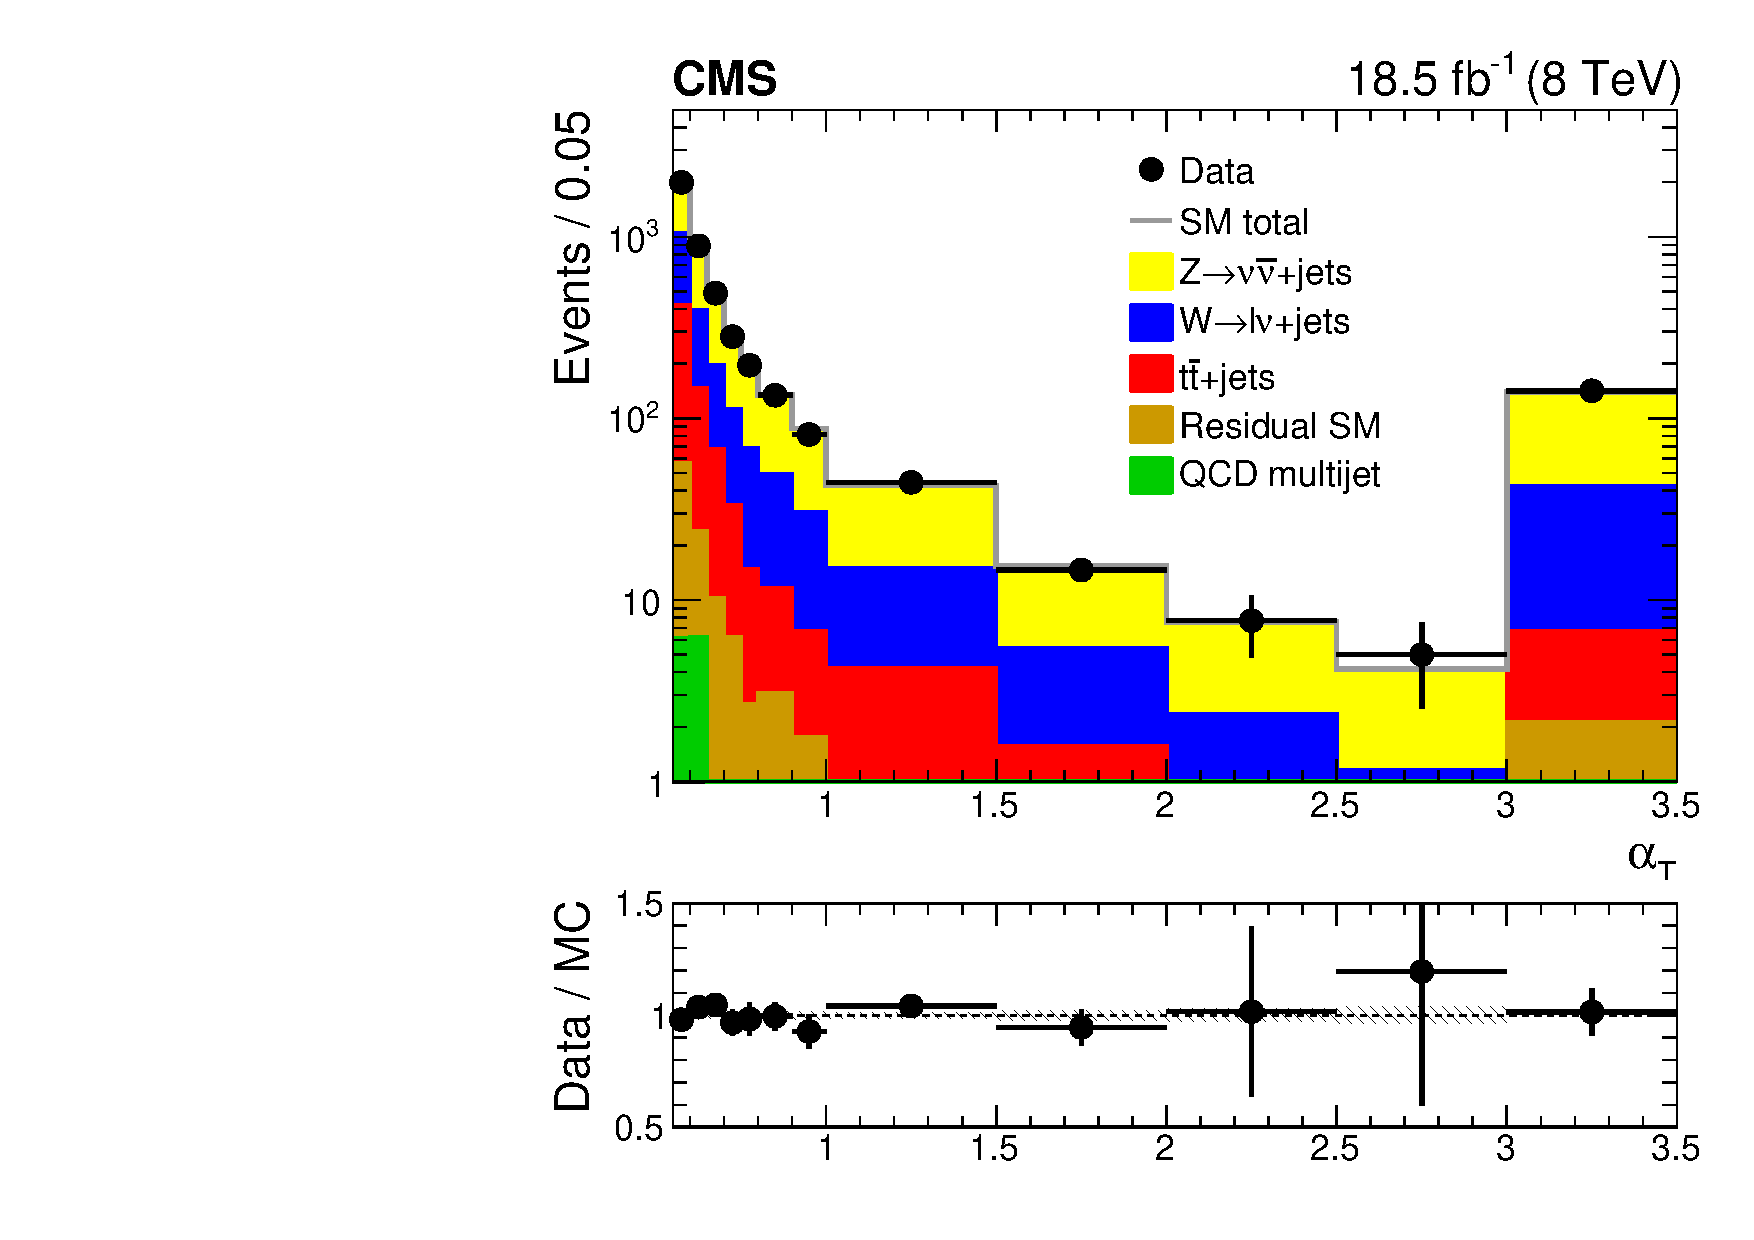
\includegraphics[width=0.7\textwidth]{AlphaT_SR} \\
    \caption{ (Upper panel) The $\alpha_\text{T}$ distribution
      observed in data for events that satisfy the full signal region
      selection criteria, including the requirements $n_\text{jet}
      \geq 2$, $n_\text{b} \geq 0$, $H_\text{T} > 375\GeV$, and
      $\alpha_\text{T} > 0.55$. Both candidate signal event yields
      observed in data (solid circles) and SM expectations as
      determined from simulation (solid histograms) are
      shown. Contributions from the SM processes of single top quark,
      diboson, Drell-Yan, and \ttbar + gauge boson (W, Z, H)
      production are collectively labelled ``Residual SM''. The final
      bin contains the overflow events.  (Lower panel) The ratios of
      the binned yields obtained from data and Monte Carlo (MC)
      simulation as a function of $\alpha_\text{T}$. The statistical
      uncertainties in the SM expectations are represented by the
      hatched areas. While the search relies only on simulation
      through ratios, this figure illustrates the accuracy of the
      simulation modelling. }
  \end{center}
\end{figure}

\clearpage
\begin{figure}[h!]
  \begin{center}
    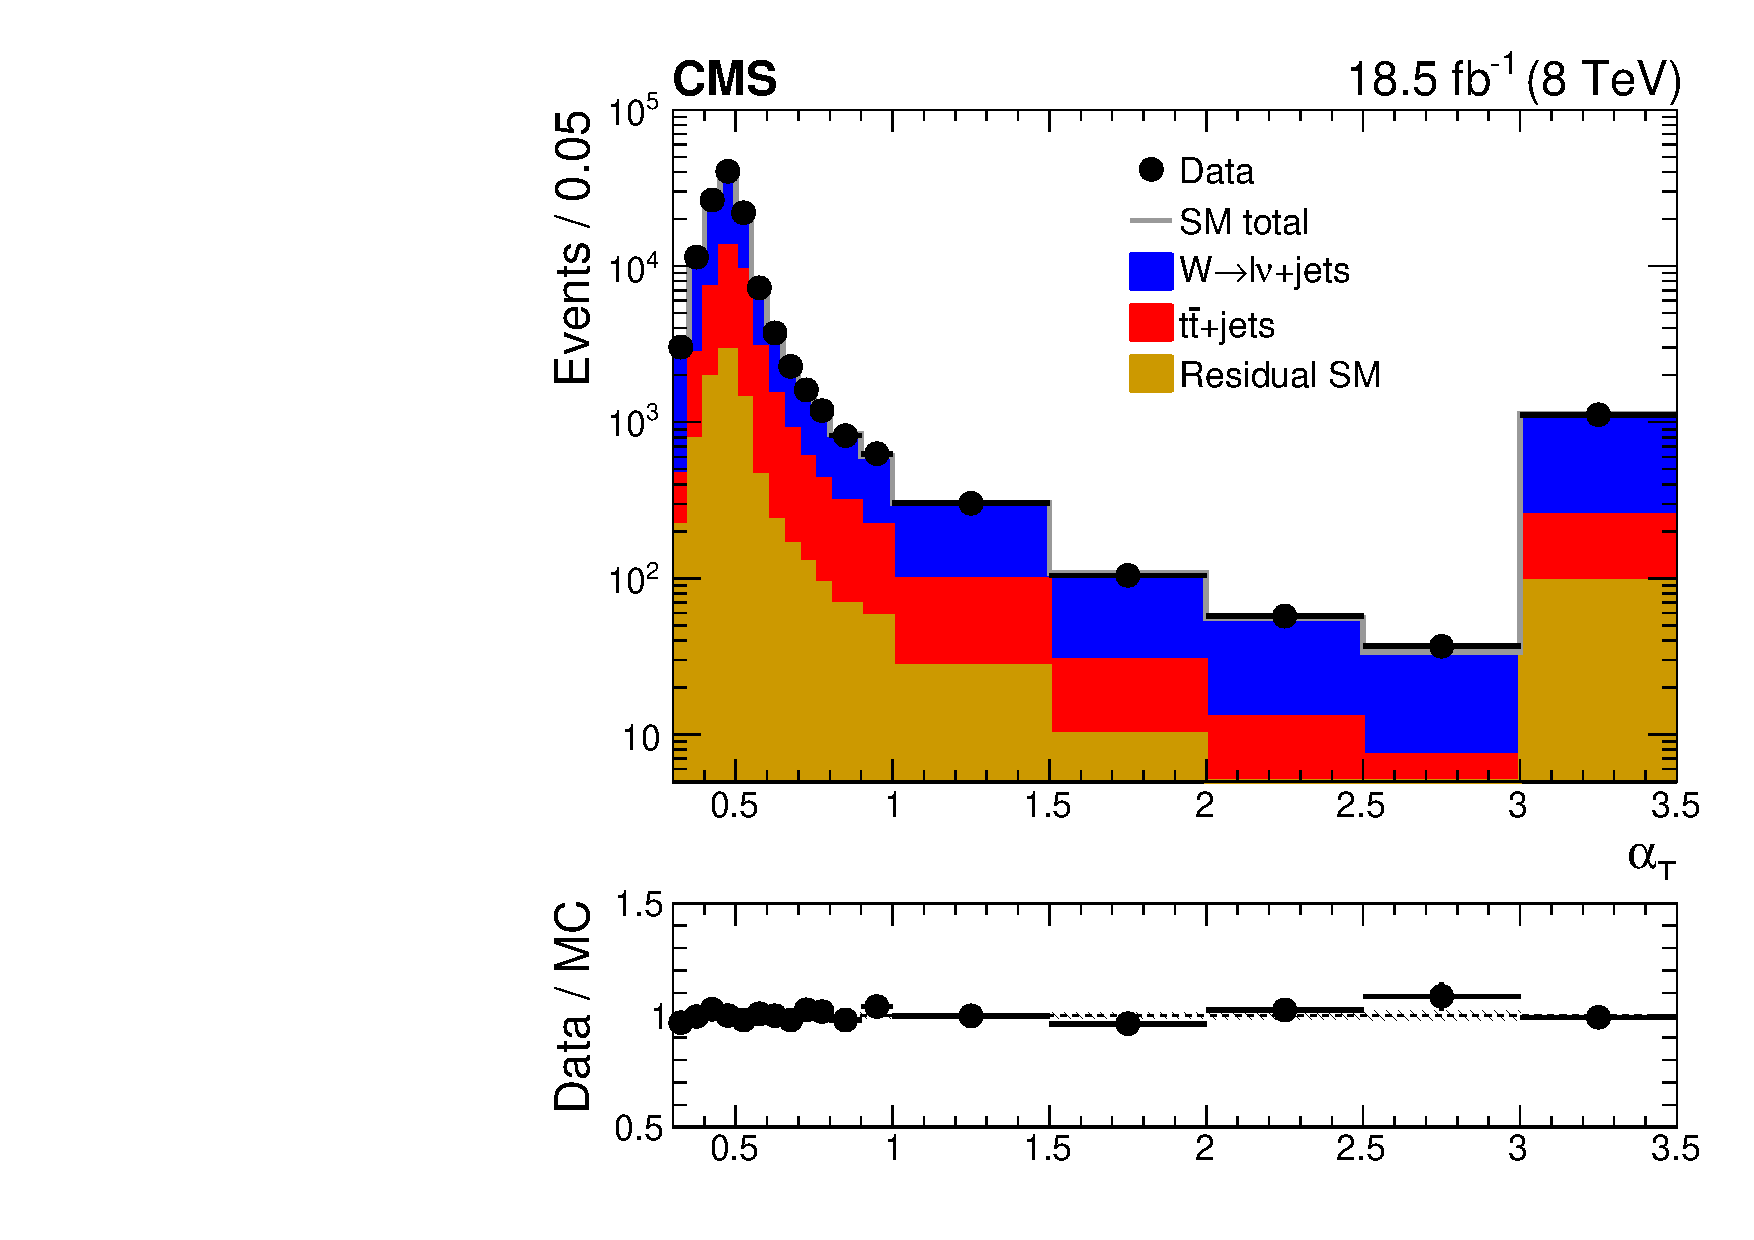
\includegraphics[width=0.7\textwidth]{AlphaT_CR} \\
    \caption{ (Upper panel) The $\alpha_\text{T}$ distribution
      observed in data for events that satisfy the selection criteria
      defining the $\mu$ + jets control region, including the
      requirements $n_\text{jet} \geq 2$, $n_\text{b} \geq 0$,
      $H_\text{T} > 200\GeV$. Event yields observed in data (solid
      circles) and SM expectations as determined from simulation
      (solid histograms) are shown. Contributions from the SM
      processes of single top quark, diboson, Drell-Yan, and \ttbar +
      gauge boson (W, Z, H) production are collectively labelled
      ``Residual SM''. The final bin contains the overflow events.
      (Lower panel) The ratios of the binned yields obtained from data
      and Monte Carlo (MC) simulation as a function of
      $\alpha_\text{T}$. The statistical uncertainties in the SM
      expectations are represented by the hatched areas. While the
      search relies only on simulation through ratios, this figure
      illustrates the accuracy of the simulation modelling. }
  \end{center}
\end{figure}

\clearpage
\newcommand{\znunu}{\ensuremath{\cPZ\rightarrow\cPgn\cPagn}\xspace}
\begin{table}[h!]
  \caption{Relative expected background contributions (\%) in the
    signal region per ($n_\text{jet}$, $n_\text{b}$) event category
    per $H_\text{T}$ bin as determined from simulation. The individual
    contributions are shown for \znunu + jets, W + jets, and
    \ttbar. Contributions from the SM processes of single top quark,
    diboson, Drell-Yan, and \ttbar + gauge boson (W, Z, H) production
    are collectively labelled ``Residual SM''. QCD multijet production
    is considered to be negligible. For each row that lists fewer than
    the full set of columns, the final entry represents values
    obtained for an open final $H_\text{T}$ bin.}   
  \centering
  \renewcommand*{\arraystretch}{1.2}
  \begin{tabular}{ llrrrrrrrrrrr }
    \hline
    ($n_\text{jet}$, \, $n_\text{b}$) & Process     & \multicolumn{11}{c}{Lower bound on $H_\text{T}$ bin (\GeVns)}    \\ 
    \cline{3-13}
                                      &             & 200 & 275 & 325 & 375 & 475 & 575 & 675 & 775 & 875 & 975 & 1075 \\ 
    \hline
    (2--3,    \, 0)                   & \znunu      & 55  & 58  & 58  & 61  & 66  & 69  & 72  & 75  & 73  & 68  & 80   \\ 
    (2--3,    \, 0)                   & W + jets    & 38  & 35  & 36  & 34  & 31  & 29  & 26  & 23  & 26  & 32  & 20   \\ 
    (2--3,    \, 0)                   & \ttbar      & 4   & 4   & 4   & 3   & 2   & 1   & 1   & 0   & 0   & 0   & 0    \\ 
    (2--3,    \, 0)                   & Residual SM & 3   & 3   & 2   & 2   & 1   & 1   & 1   & 2   & 1   & 0   & 0    \\ 
    (2--3,    \, 1)                   & \znunu      & 35  & 36  & 36  & 39  & 49  & 56  & 62  & 68  & 77  & 61  & 71   \\ 
    (2--3,    \, 1)                   & W + jets    & 20  & 19  & 20  & 19  & 22  & 22  & 21  & 24  & 19  & 37  & 29   \\ 
    (2--3,    \, 1)                   & \ttbar      & 37  & 38  & 38  & 37  & 25  & 18  & 14  & 6   & 4   & 0   & 0    \\ 
    (2--3,    \, 1)                   & Residual SM & 7   & 7   & 6   & 5   & 4   & 4   & 3   & 2   & 0   & 2   & 0    \\ 
    (2--3,    \, 2)                   & \znunu      & 28  & 22  & 17  & 18  & 24  & 28  & 29  & 78  & 52               \\ 
    (2--3,    \, 2)                   & W + jets    & 11  & 8   & 7   & 6   & 7   & 11  & 10  & 11  & 5                \\ 
    (2--3,    \, 2)                   & \ttbar      & 51  & 63  & 68  & 70  & 64  & 53  & 57  & 7   & 43               \\ 
    (2--3,    \, 2)                   & Residual SM & 10  & 7   & 8   & 6   & 5   & 8   & 4   & 4   & 0                \\ 
    ($\geq4$, \, 0)                   & \znunu      & 47  & 46  & 44  & 46  & 51  & 57  & 61  & 58  & 66  & 68  & 60   \\ 
    ($\geq4$, \, 0)                   & W + jets    & 34  & 36  & 36  & 35  & 33  & 32  & 30  & 33  & 27  & 25  & 31   \\ 
    ($\geq4$, \, 0)                   & \ttbar      & 15  & 15  & 17  & 16  & 13  & 9   & 8   & 8   & 6   & 6   & 7    \\ 
    ($\geq4$, \, 0)                   & Residual SM & 4   & 3   & 3   & 3   & 3   & 2   & 1   & 1   & 1   & 1   & 2    \\ 
    ($\geq4$, \, 1)                   & \znunu      & 17  & 17  & 14  & 16  & 19  & 25  & 33  & 36  & 34  & 39  & 39   \\ 
    ($\geq4$, \, 1)                   & W + jets    & 12  & 12  & 10  & 11  & 12  & 13  & 13  & 17  & 16  & 14  & 16   \\ 
    ($\geq4$, \, 1)                   & \ttbar      & 66  & 67  & 72  & 69  & 63  & 56  & 50  & 42  & 49  & 45  & 45   \\ 
    ($\geq4$, \, 1)                   & Residual SM & 5   & 4   & 4   & 4   & 6   & 6   & 4   & 5   & 1   & 2   & 0    \\ 
    ($\geq4$, \, 2)                   & \znunu      & 7   & 7   & 5   & 6   & 6   & 8   & 14  & 16  & 9                \\ 
    ($\geq4$, \, 2)                   & W + jets    & 6   & 4   & 2   & 3   & 3   & 4   & 3   & 7   & 4                \\ 
    ($\geq4$, \, 2)                   & \ttbar      & 83  & 85  & 88  & 87  & 85  & 83  & 80  & 75  & 86               \\ 
    ($\geq4$, \, 2)                   & Residual SM & 4   & 4   & 5   & 4   & 5   & 6   & 3   & 2   & 1                \\ 
    ($\geq4$, \, 3)                   & \znunu      & 2   & 3   & 2   & 3   & 3   & 3   & 8   & 8   & 6                \\ 
    ($\geq4$, \, 3)                   & W + jets    & 3   & 2   & 1   & 1   & 1   & 2   & 1   & 3   & 0                \\ 
    ($\geq4$, \, 3)                   & \ttbar      & 90  & 92  & 92  & 93  & 91  & 91  & 88  & 89  & 91               \\ 
    ($\geq4$, \, 3)                   & Residual SM & 5   & 3   & 5   & 3   & 5   & 4   & 3   & 0   & 3                \\ 
    ($\geq4$, \, $\geq4$)             & \znunu      & 0   & 6   & 0   & 0                                              \\ 
    ($\geq4$, \, $\geq4$)             & W + jets    & 0   & 0   & 0   & 0                                              \\ 
    ($\geq4$, \, $\geq4$)             & \ttbar      & 100 & 88  & 94  & 95                                             \\ 
    ($\geq4$, \, $\geq4$)             & Residual SM & 0   & 6   & 6   & 5                                              \\ 
    \hline
  \end{tabular}
\end{table}

%\clearpage
%\begin{table}[h!]
%  \caption{Control samples used to predict the SM
%    backgrounds for each event category. }
%  \label{tab:fit-plots}
%  \centering
%  \renewcommand*{\arraystretch}{1.2}
%  \begin{tabular}{ ll }
%    \hline
%    ($n_\text{jet}$, \, $n_\text{b}$ & Control samples                                \\ 
%    \hline
%    (2--3, \, 0)                     & $\mu$ + jets, $\mu\mu$ + jets, $\gamma$ + jets \\
%    (2--3, \, 1)                     & $\mu$ + jets, $\mu\mu$ + jets, $\gamma$ + jets \\
%    (2--3, \, 2)                     & $\mu$ + jets                                   \\
%    ($\geq4$, \, 0)                  & $\mu$ + jets, $\mu\mu$ + jets, $\gamma$ + jets \\
%    ($\geq4$, \, 1)                  & $\mu$ + jets, $\mu\mu$ + jets, $\gamma$ + jets \\
%    ($\geq4$, \, 2)                  & $\mu$ + jets                                   \\
%    ($\geq4$, \, 3)                  & $\mu$ + jets                                   \\
%    ($\geq4$, \, $\geq4$)            & $\mu$ + jets                                   \\
%    \hline
%  \end{tabular}
%\end{table}

\clearpage
\begin{table}[h!]
  \caption{
    Binned yields in the $\mu$ + jets control sample, for events
    categorised according to $n_\text{jet}$, $n_\text{b}$, and
    $H_\text{T}$, and the corresponding SM expectations (labelled 
    ``SM'') as obtained from a combined fit to the control and signal
    regions under the background-only hypothesis. 
    The quoted uncertainties include both statistical and systematic  
    components. For each row that lists fewer than the full set of 
    columns, the final entry represents values obtained for an open
    final $H_\text{T}$ bin. 
  }
  \centering
  \resizebox{\textwidth}{!}{
    \renewcommand*{\arraystretch}{1.4}
    \begin{tabular}{ lllllllllllll }
      \hline
      Category & $\mu$ + jets & \multicolumn{11}{c}{$H_\text{T}$ (\GeVns)} \\
      \cline{3-13}
      ($n_\text{jet}$,\,$n_\text{b}$)
               & sample 
               & 200--275
               & 275--325
               & 325--375
               & 375--475
               & 475--575
               & 575--675
               & 675--775
               & 775--875
               & 875--975
               & 975--1075
               & 1075--$\infty$                                            \\
               \hline
               (2--3,\,0)
               & Data
               & $43530$
               & $16470$
               & $8791$
               & $8195$
               & $3226$
               & $1429$
               & $582$
               & $317$
               & $128$
               & $75$
               & $128$                                                     \\
               (2--3,\,0)
               & SM
               & $43560^{+160}_{-230}$ % $43555^{+163}_{-225}$
               & $16460^{+100}_{-140}$ % $16463^{+103}_{-142}$
               & $8792^{+76}_{-83}$
               & $8186^{+101}_{-93}$
               & $3231^{+49}_{-63}$
               & $1425^{+34}_{-37}$
               & $584^{+26}_{-17}$
               & $318^{+22}_{-14}$
               & $128^{+11}_{-11}$
               & $75.8^{+8.5}_{-9.3}$
               & $127^{+15}_{-10}$                             \\\\[-2ex]
               (2--3,\,1)
               & Data
               & $10590$
               & $4334$
               & $2300$
               & $2129$
               & $720$
               & $269$
               & $113$
               & $51$
               & $21$
               & $12$
               & $20$                                          \\
               (2--3,\,1)
               & SM         
               & $10600^{+120}_{-60}$ % $10604^{+122}_{-62}$
               & $4330^{+66}_{-55}$
               & $2300^{+54}_{-44}$
               & $2120^{+48}_{-42}$
               & $720^{+29}_{-33}$
               & $271^{+14}_{-17}$
               & $112^{+7}_{-13}$
               & $51.4^{+5.7}_{-7.6}$
               & $20.9^{+5.0}_{-4.0}$
               & $11.9^{+5.0}_{-3.0}$
               & $20.2^{+4.7}_{-3.3}$                          \\\\[-2ex]
               (2--3,\,2)
               & Data
               & $3065$
               & $1410$
               & $773$
               & $642$
               & $202$
               & $62$
               & $21$
               & $11$
               & $7$                                           \\
               (2--3,\,2)
               & SM
               & $3054^{+42}_{-57}$
               & $1409^{+28}_{-36}$
               & $775^{+30}_{-19}$
               & $637^{+24}_{-24}$
               & $206^{+16}_{-12}$
               & $67.7^{+6.6}_{-8.9}$
               & $20.3^{+4.9}_{-4.9}$
               & $10.8^{+3.9}_{-3.0}$
               & $6.9^{+2.0}_{-2.9}$                           \\\\[-2ex]
               ($\geq4$,\,0)
               & Data
               & $641$
               & $2128$
               & $1007$
               & $1013$
               & $715$
               & $471$
               & $252$
               & $133$
               & $66$
               & $42$
               & $55$                                          \\
               ($\geq4$,\,0)
               & SM
               & $639^{+25}_{-29}$
               & $2140^{+47}_{-41}$
               & $1008^{+21}_{-35}$
               & $1012^{+37}_{-34}$
               & $719^{+29}_{-25}$
               & $476^{+21}_{-19}$
               & $250^{+16}_{-13}$
               & $132^{+12}_{-10}$
               & $66.4^{+8.5}_{-6.6}$
               & $42.1^{+6.1}_{-6.6}$
               & $56.0^{+8.1}_{-8.0}$                          \\\\[-2ex]
               ($\geq4$,\,1)
               & Data
               & $570$
               & $2034$
               & $913$
               & $1016$
               & $720$
               & $321$
               & $163$
               & $77$
               & $38$
               & $24$
               & $23$                                          \\
               ($\geq4$,\,1)
               & SM
               & $569^{+23}_{-24}$
               & $2025^{+44}_{-39}$
               & $914^{+31}_{-33}$
               & $1018^{+32}_{-28}$
               & $723^{+24}_{-25}$
               & $323^{+19}_{-17}$
               & $161^{+15}_{-14}$
               & $78.3^{+7.3}_{-8.2}$
               & $38.6^{+5.2}_{-6.4}$
               & $24.0^{+5.5}_{-4.8}$
               & $23.0^{+5.0}_{-4.0}$                          \\\\[-2ex]
               ($\geq4$,\,2)
               & Data
               & $339$
               & $1265$
               & $642$
               & $678$
               & $471$
               & $232$
               & $116$
               & $42$
               & $43$                                          \\
               ($\geq4$,\,2)
               & SM
               & $342^{+21}_{-15}$
               & $1268^{+37}_{-41}$
               & $640^{+26}_{-25}$
               & $676^{+21}_{-30}$
               & $478^{+22}_{-21}$
               & $235^{+19}_{-14}$
               & $117^{+8}_{-9}$
               & $42.0^{+6.8}_{-7.7}$
               & $43.3^{+5.9}_{-5.6}$                          \\\\[-2ex]
               ($\geq4$,\,3)
               & Data
               & $41$
               & $153$
               & $75$
               & $86$
               & $59$
               & $28$
               & $16$
               & $5$
               & $6$                                           \\
               ($\geq4$,\,3)
               & SM
               & $39.9^{+5.1}_{-7.4}$
               & $152^{+12}_{-11}$
               & $70.2^{+7.8}_{-7.5}$
               & $83.8^{+10.9}_{-6.5}$
               & $60.9^{+7.7}_{-6.9}$
               & $27.9^{+5.1}_{-5.8}$
               & $16.6^{+4.8}_{-4.0}$
               & $4.9^{+2.1}_{-2.0}$
               & $5.9^{+2.9}_{-2.0}$                           \\\\[-2ex]
               ($\geq4$,\,$\geq4$)
               & Data
               & $0$
               & $3$
               & $3$
               & $8$                                           \\
               ($\geq4$,\,$\geq4$)
               & SM
               & $<0.1$ % $0.0^{+0.0}_{-0.0}$
               & $2.8^{+1.0}_{-1.0}$
               & $2.6^{+1.7}_{-1.7}$
               & $9.6^{+2.9}_{-2.9}$                           \\\\[-3ex]
     \hline
   \end{tabular}
 }
\end{table}

\clearpage
\begin{table}[h!]
  \caption{
    Binned yields in the $\mu\mu$ + jets control sample, for events
    categorised according to $n_\text{jet}$, $n_\text{b}$, and
    $H_\text{T}$, and the corresponding SM expectations (labelled 
    ``SM'') as obtained from a combined fit to the control and signal
    regions under the background-only hypothesis. 
    The quoted uncertainties include both statistical and systematic  
    components. For each row that lists fewer than the full set of 
    columns, the final entry represents values obtained for an open
    final $H_\text{T}$ bin. 
  }
  \centering
  \resizebox{\textwidth}{!}{
    \renewcommand*{\arraystretch}{1.4}
    \begin{tabular}{ lllllllllllll }
      \hline
      Category & $\mu\mu$ + jets & \multicolumn{11}{c}{$H_\text{T}$ (\GeVns)} \\
      \cline{3-13}
      ($n_\text{jet}$,\,$n_\text{b}$)
               & sample
               & 200--275
               & 275--325
               & 325--375
               & 375--475
               & 475--575
               & 575--675
               & 675--775
               & 775--875
               & 875--975
               & 975--1075
               & 1075--$\infty$                                               \\
               \hline
               (2--3,\,0)
               & Data 
               & $3096$
               & $1385$
               & $722$
               & $729$
               & $283$
               & $129$
               & $57$
               & $28$
               & $13$
               & $10$
               & $8$                                                          \\
               (2--3,\,0)
               & SM
               & $3126^{+52}_{-62}$
               & $1375^{+30}_{-38}$
               & $724^{+26}_{-20}$
               & $718^{+21}_{-19}$
               & $291^{+12}_{-7}$
               & $129^{+9}_{-10}$
               & $55.8^{+4.9}_{-5.5}$
               & $27.4^{+3.6}_{-3.9}$
               & $13.5^{+2.6}_{-2.6}$
               & $8.4^{+1.9}_{-2.2}$
               & $11.1^{+2.2}_{-3.5}$                                         \\\\[-2ex]
               (2--3,\,1)
               & Data
               & $448$
               & $217$
               & $102$
               & $112$
               & $38$
               & $16$
               & $8$
               & $3$
               & $5$
               & $1$
               & $1$                                                          \\
               (2--3,\,1)
               & SM         
               & $456^{+17}_{-24}$
               & $214^{+11}_{-16}$
               & $102^{+6}_{-10}$
               & $108^{+7}_{-7}$
               & $42.2^{+4.2}_{-4.0}$
               & $15.0^{+2.0}_{-2.8}$
               & $8.4^{+1.4}_{-2.0}$
               & $3.1^{+0.8}_{-1.0}$
               & $3.5^{+1.4}_{-1.0}$
               & $0.4^{+0.5}_{-0.4}$
               & $0.8^{+0.4}_{-0.8}$                                          \\\\[-2ex]
               ($\geq4$,\,0)
               & Data
               & $34$
               & $107$
               & $46$
               & $61$
               & $54$
               & $28$
               & $16$
               & $5$
               & $5$
               & $2$
               & $2$                                                          \\
               ($\geq4$,\,0)
               & SM
               & $31.7^{+3.2}_{-4.3}$
               & $118^{+10}_{-10}$
               & $46.4^{+5.5}_{-5.8}$
               & $61.8^{+4.1}_{-5.0}$
               & $54.1^{+4.4}_{-4.3}$
               & $30.3^{+4.7}_{-3.8}$
               & $16.5^{+2.5}_{-2.6}$
               & $6.7^{+1.2}_{-1.7}$
               & $4.9^{+1.4}_{-1.4}$
               & $2.7^{+1.0}_{-1.1}$
               & $3.7^{+1.5}_{-1.1}$                                          \\\\[-2ex]
               ($\geq4$,\,1)
               & Data
               & $9$
               & $34$
               & $19$
               & $27$
               & $10$
               & $12$
               & $2$
               & $3$
               & $2$
               & $0$
               & $1$                                                          \\
               ($\geq4$,\,1)
               & SM
               & $8.8^{+2.0}_{-3.6}$
               & $32.0^{+5.3}_{-5.1}$
               & $19.2^{+4.5}_{-4.3}$
               & $21.9^{+3.1}_{-2.1}$
               & $15.3^{+2.4}_{-2.3}$
               & $9.8^{+2.1}_{-1.6}$
               & $3.8^{+1.4}_{-0.9}$
               & $4.3^{+1.1}_{-1.4}$
               & $1.8^{+0.7}_{-0.8}$
               & $1.2^{+0.5}_{-0.6}$
               & $2.2^{+0.8}_{-1.2}$                                          \\\\[-3ex]
      \hline
   \end{tabular}
 }
\end{table}

\clearpage
\begin{table}[h!]
  \caption{
    Binned yields in the $\gamma$ + jets control sample, for events
    categorised according to $n_\text{jet}$, $n_\text{b}$, and
    $H_\text{T}$, and the corresponding SM expectations (labelled 
    ``SM'') as obtained from a combined fit to the control and signal
    regions under the background-only hypothesis. 
    The quoted uncertainties include both statistical and systematic  
    components. For each row that lists fewer than the full set of 
    columns, the final entry represents values obtained for an open
    final $H_\text{T}$ bin. 
  }
  \centering
  \resizebox{\textwidth}{!}{
    \renewcommand*{\arraystretch}{1.4}
    \begin{tabular}{ lllllllllllll }
      \hline
      Category & $\gamma$ + jets & \multicolumn{11}{c}{$H_\text{T}$ (\GeVns)} \\
      \cline{3-13}
      ($n_\text{jet}$,\,$n_\text{b}$)
               & sample
               & 200--275
               & 275--325
               & 325--375
               & 375--475
               & 475--575
               & 575--675
               & 675--775
               & 775--875
               & 875--975
               & 975--1075
               & 1075--$\infty$                                               \\
               \hline
               (2--3,\,0)
               & Data
               & --                             
               & --                       
               & --                     
               & $3522$
               & $1068$
               & $395$
               & $129$
               & $45$
               & $19$
               & $9$
               & $14$                                                         \\
               (2--3,\,0)
               & SM
               & --                          
               & --                          
               & --             
               & $3517^{+45}_{-76}$
               & $1071^{+32}_{-26}$
               & $387^{+19}_{-24}$
               & $135^{+8}_{-10}$
               & $46.9^{+5.2}_{-6.2}$
               & $18.2^{+3.6}_{-2.9}$
               & $13.1^{+3.1}_{-3.2}$
               & $9.1^{+1.5}_{-2.3}$                                          \\\\[-2ex]
               (2--3,\,1)
               & Data
               & --                      
               & --                   
               & --                 
               & $452$
               & $143$
               & $37$
               & $19$
               & $4$
               & $5$
               & $0$
               & $0$                                                          \\
               (2--3,\,1)
               & SM     
               & --                         
               & --                         
               & --      
               & $448^{+18}_{-14}$
               & $138^{+10}_{-10}$
               & $41.2^{+6.1}_{-5.9}$
               & $16.8^{+2.5}_{-3.8}$
               & $4.6^{+1.5}_{-1.3}$
               & $5.4^{+1.9}_{-1.6}$
               & $0.5^{+0.5}_{-0.5}$
               & $0.7^{+0.3}_{-0.7}$                                          \\\\[-2ex]
               ($\geq4$,\,0)
               & Data
               & --           
               & --  
               & --    
               & $372$
               & $251$
               & $137$
               & $71$
               & $26$
               & $13$
               & $6$
               & $6$                                                          \\
               ($\geq4$,\,0)
               & SM
               & --                          
               & --                          
               & --        
               & $371^{+18}_{-15}$
               & $256^{+16}_{-12}$
               & $142^{+11}_{-12}$
               & $67.5^{+5.0}_{-6.4}$
               & $23.6^{+3.2}_{-5.3}$
               & $14.2^{+3.0}_{-2.6}$
               & $5.7^{+1.8}_{-1.7}$
               & $6.0^{+2.3}_{-1.8}$                                          \\\\[-2ex]
               ($\geq4$,\,1)
               & Data
               & --       
               & --       
               & --           
               & $83$
               & $53$
               & $30$
               & $13$
               & $8$
               & $3$
               & $3$
               & $3$                                                          \\
               ($\geq4$,\,1)
               & SM
               & --                    
               & --        
               & --        
               & $88.7^{+8.1}_{-6.8}$
               & $48.6^{+5.4}_{-6.8}$
               & $33.7^{+5.6}_{-4.9}$
               & $10.0^{+3.9}_{-2.3}$
               & $9.2^{+2.2}_{-2.8}$
               & $4.3^{+1.6}_{-1.8}$
               & $1.9^{+0.9}_{-1.0}$
               & $1.9^{+0.9}_{-1.0}$                                          \\\\[-3ex]
      \hline
   \end{tabular}
 }
\end{table}

\clearpage
\begin{figure}[h!]
  \begin{center}
    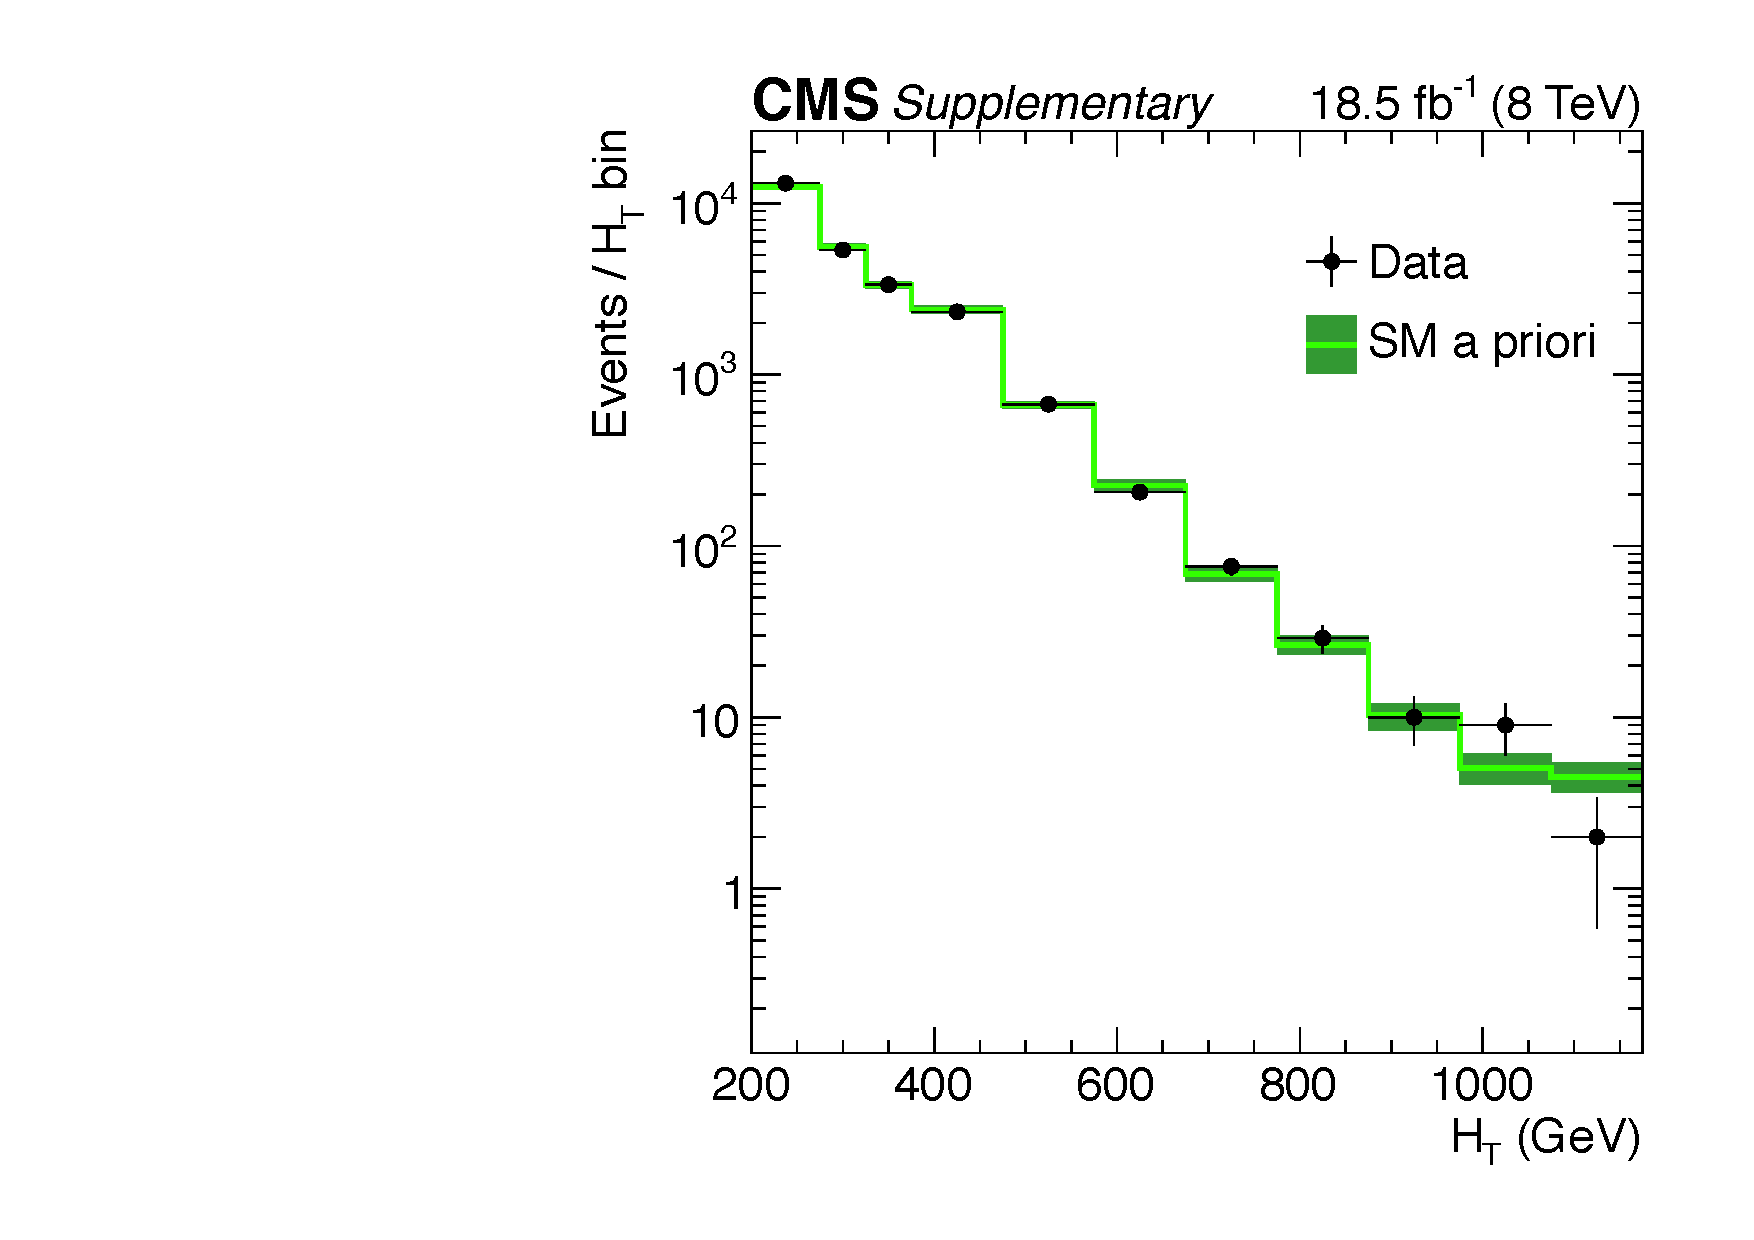
\includegraphics[width=0.7\textwidth]{eq0b_le3j_prefit_log} 
    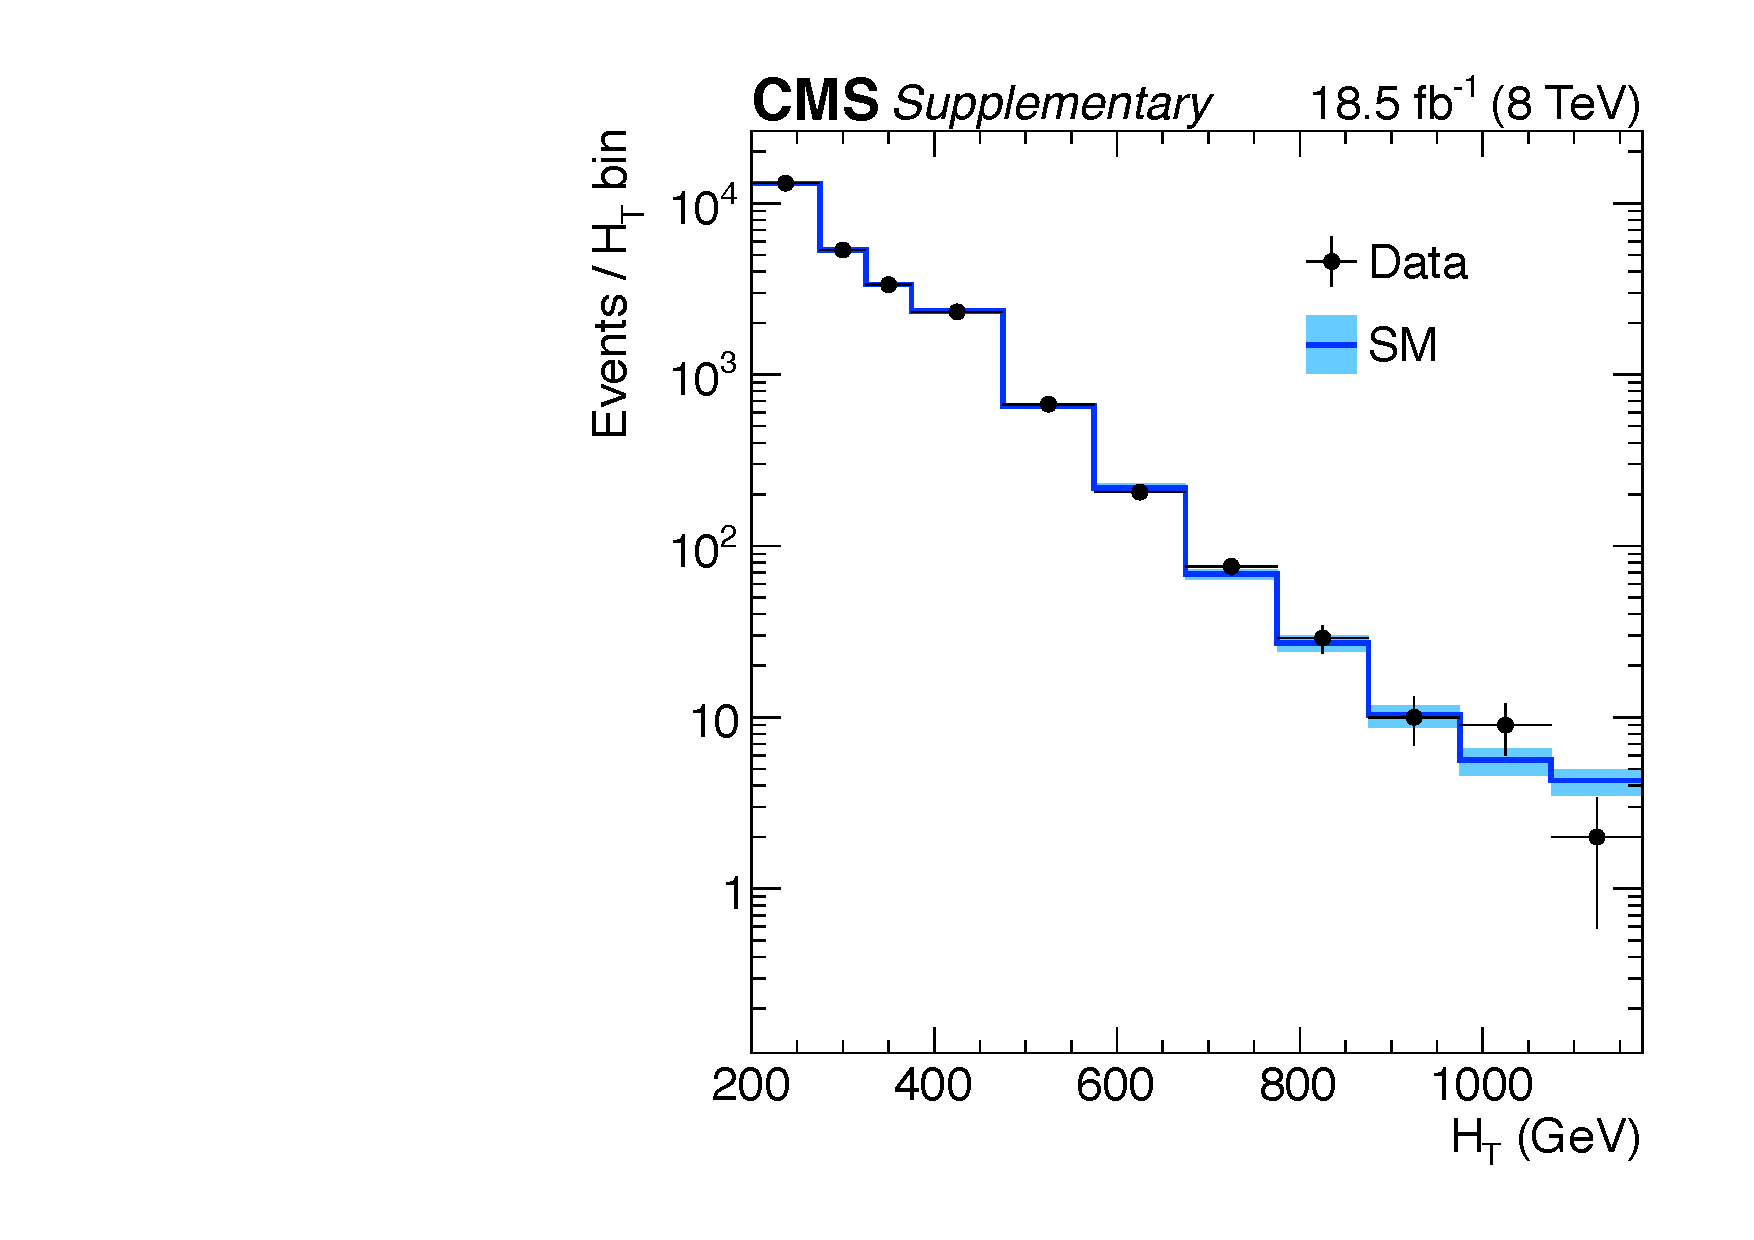
\includegraphics[width=0.7\textwidth]{eq0b_le3j_postfit_log} \\
    \caption{Candidate signal event yields observed in data (solid
      circles) and SM expectations with their associated uncertainties
      (solid lines with bands) in bins of $H_\text{T}$ for events that
      satisfy $2 \geq n_\text{jet} \geq 3$ and $n_\text{b} = 0$. (a)
      SM a priori expectations. (b) SM expectations from the fit
      including the signal region. }
  \end{center}
\end{figure}

\clearpage
\begin{figure}[h!]
  \begin{center}
    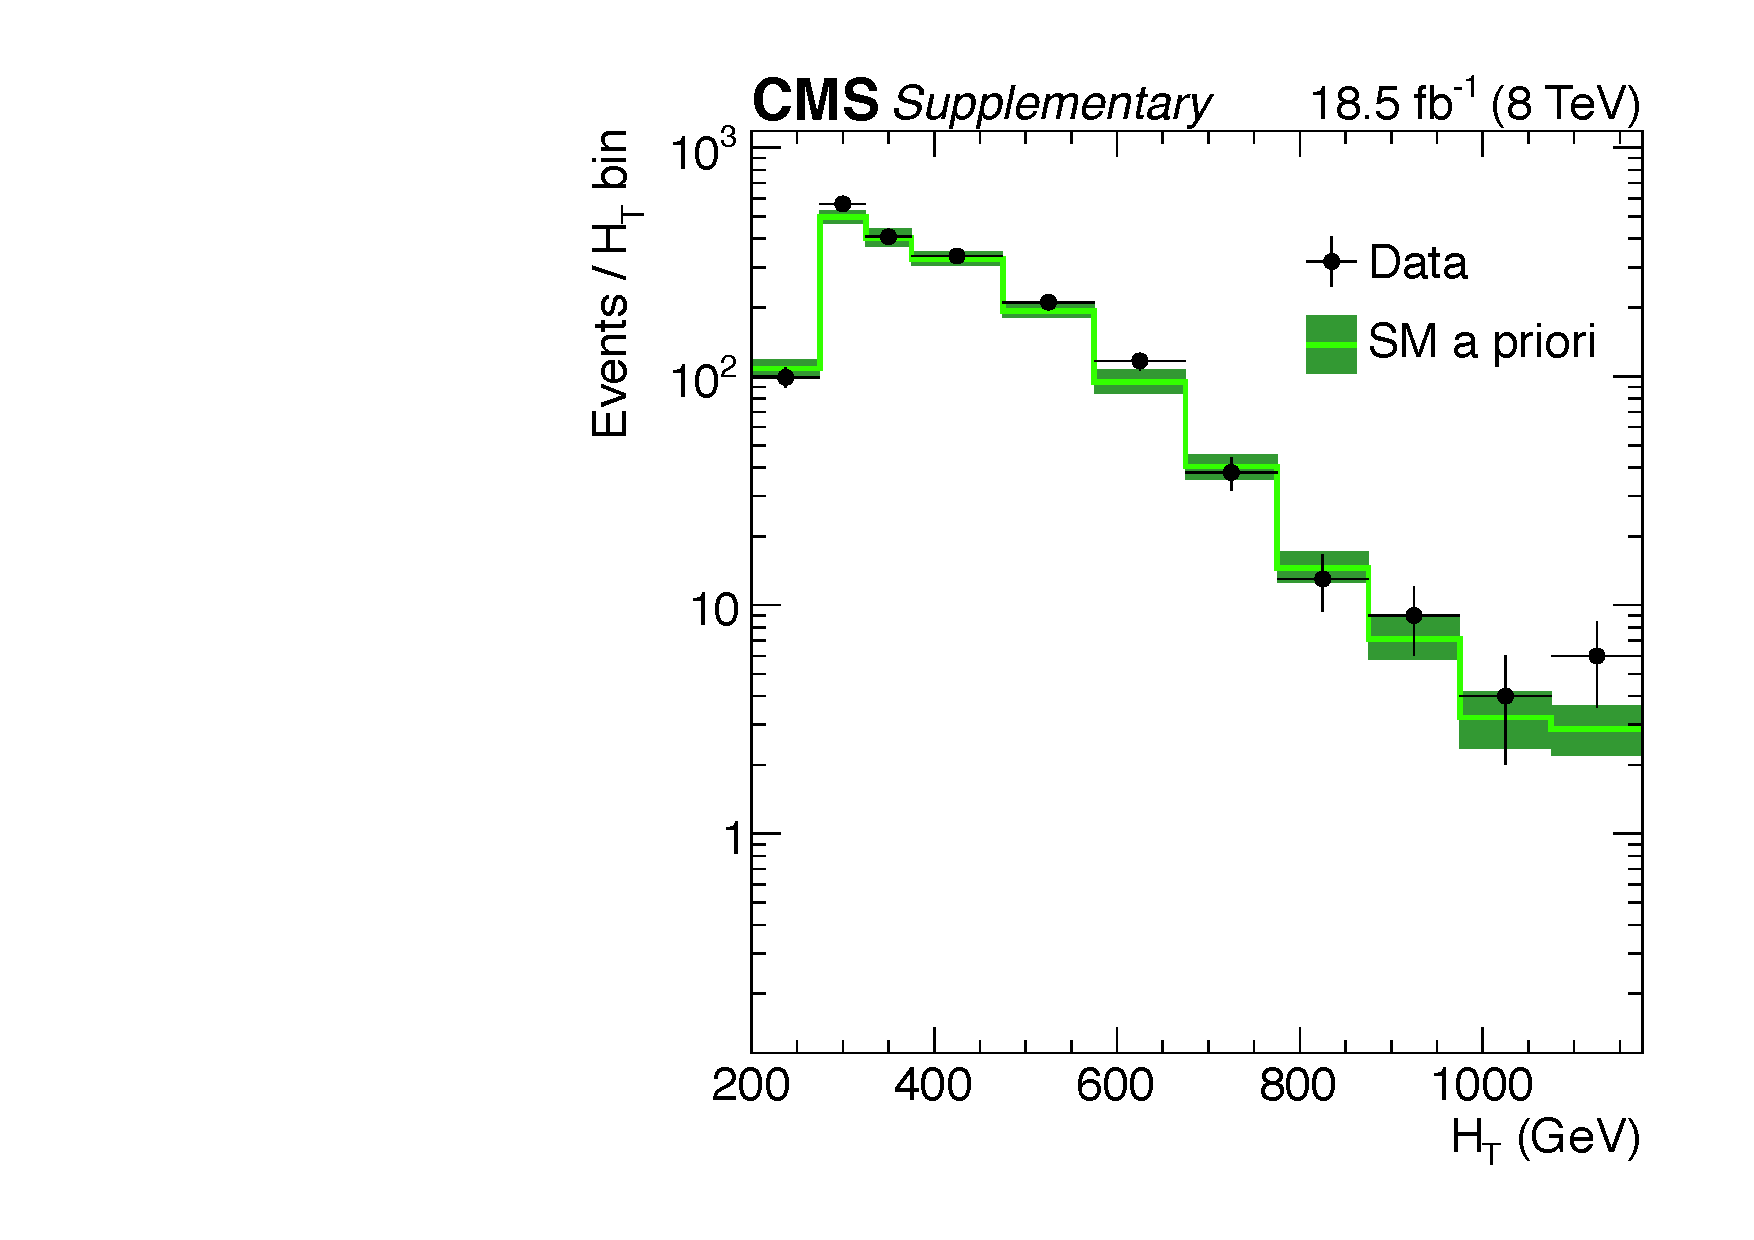
\includegraphics[width=0.7\textwidth]{eq0b_ge4j_prefit_log} 
    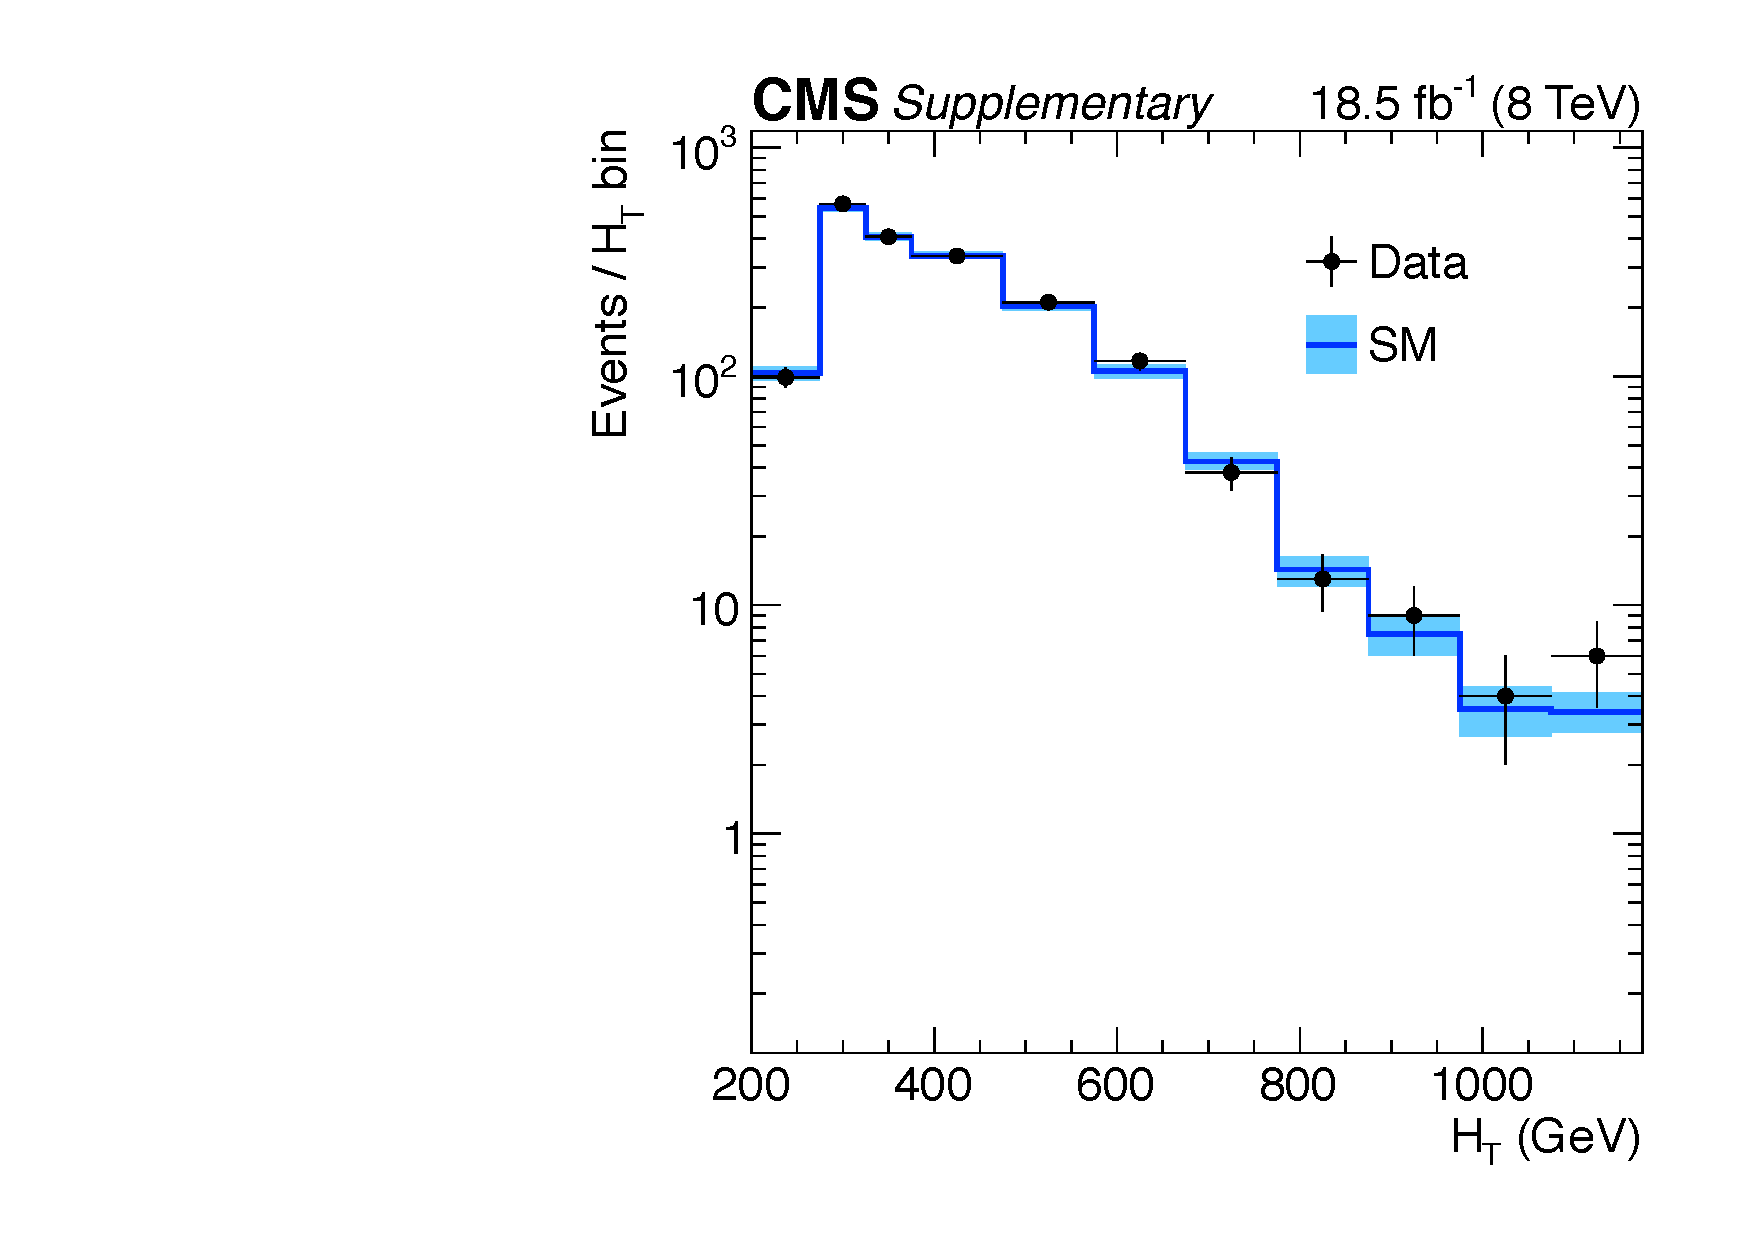
\includegraphics[width=0.7\textwidth]{eq0b_ge4j_postfit_log} \\
    \caption{Candidate signal event yields observed in data (solid
      circles) and SM expectations with their associated uncertainties
      (solid lines with bands) in bins of $H_\text{T}$ for events that
      satisfy $n_\text{jet} \geq 4$ and $n_\text{b} = 0$. (a) SM a
      priori expectations. (b) SM expectations from the fit including
      the signal region. }
  \end{center}
\end{figure}

\clearpage
\begin{figure}[h!]
  \begin{center}
    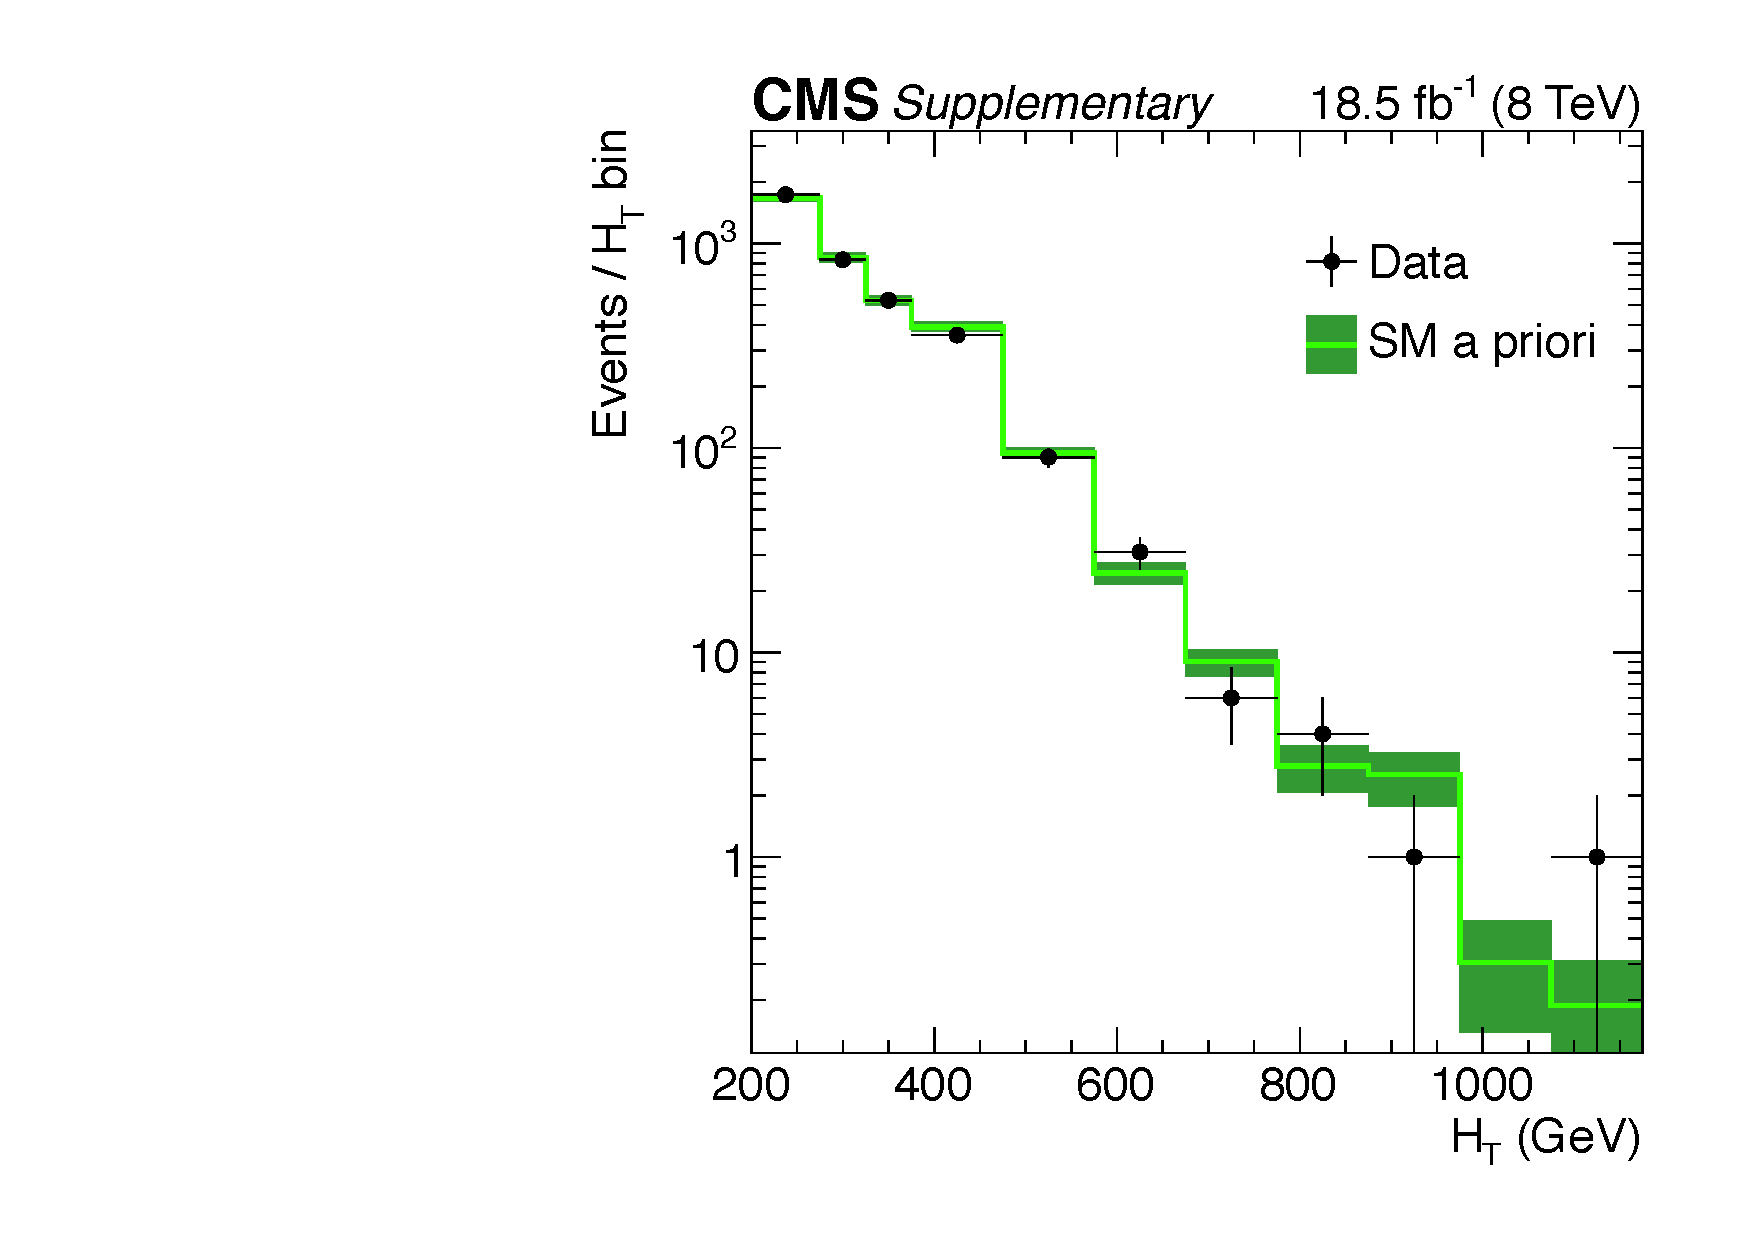
\includegraphics[width=0.7\textwidth]{eq1b_le3j_prefit_log} 
    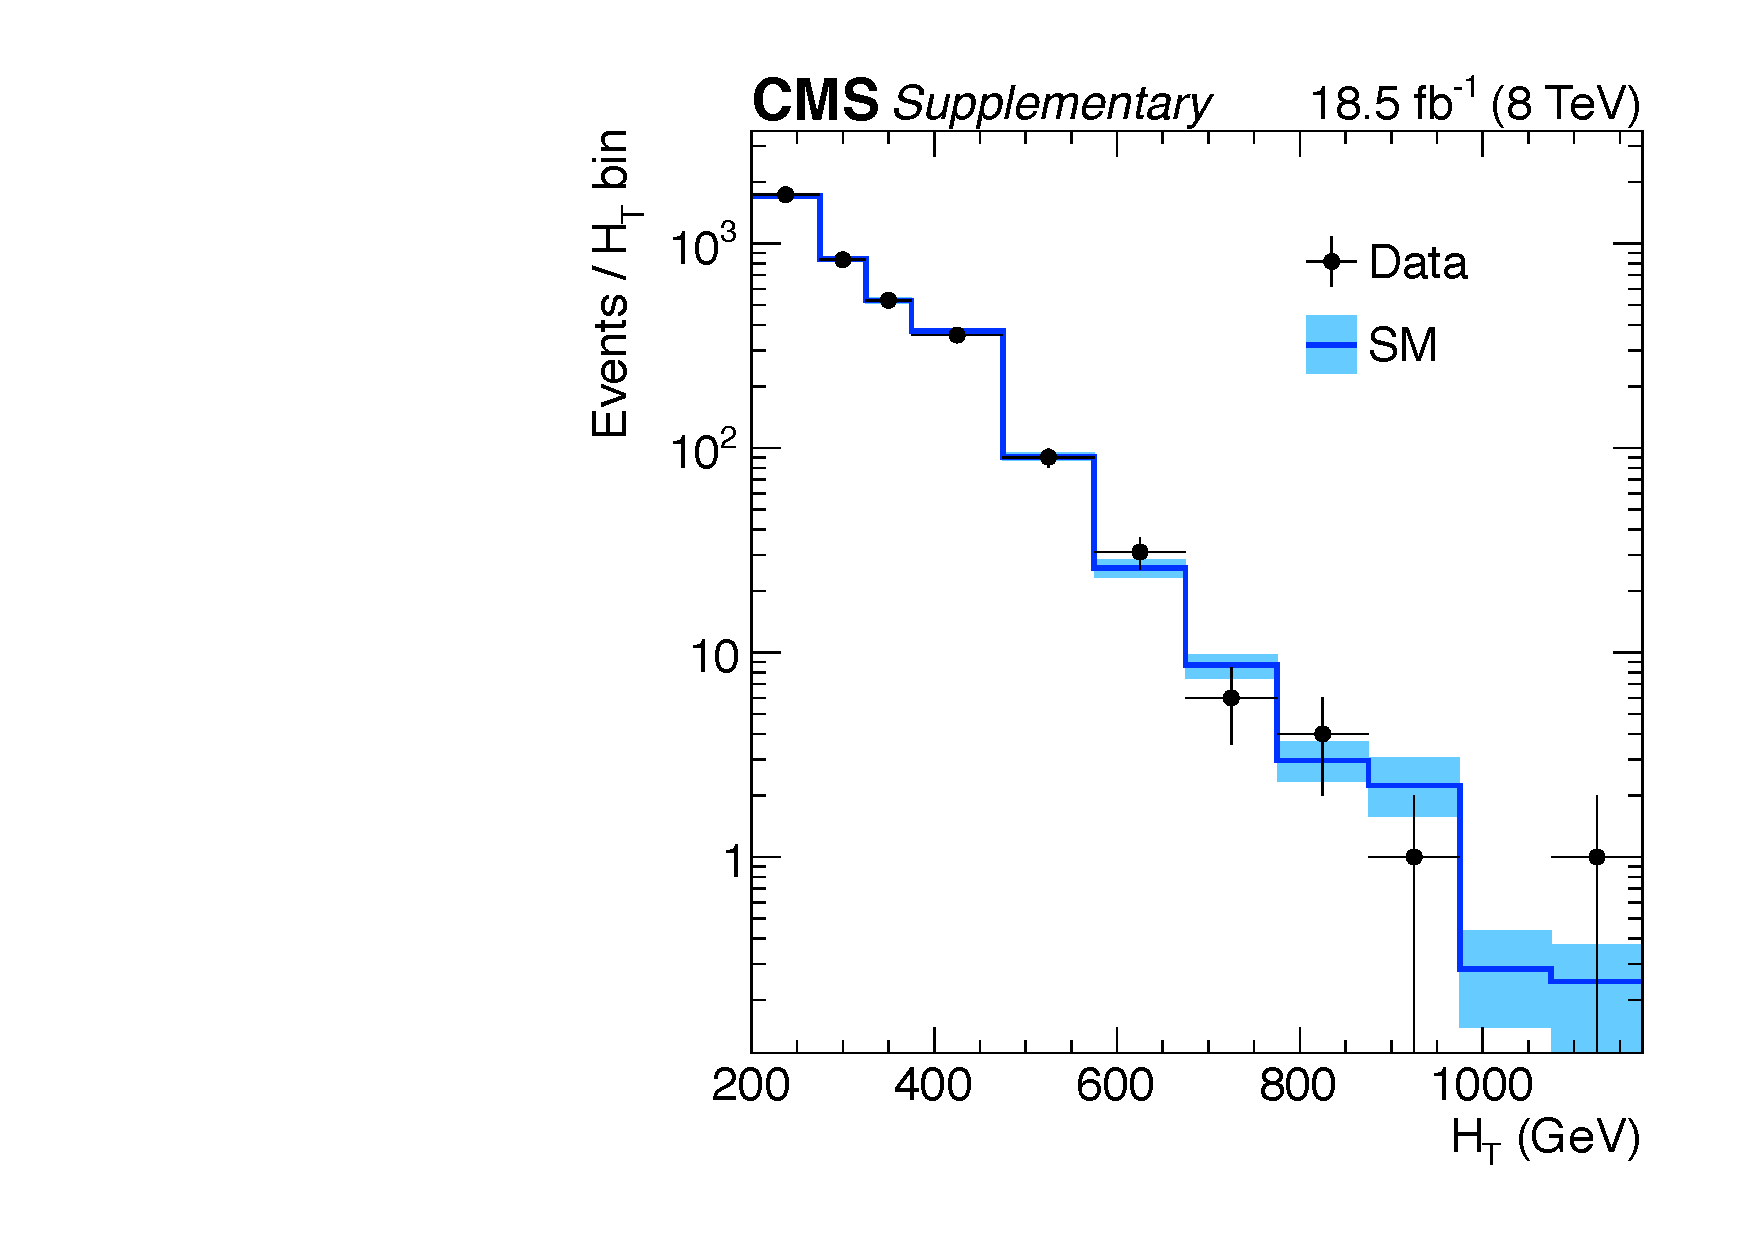
\includegraphics[width=0.7\textwidth]{eq1b_le3j_postfit_log} \\
    \caption{Candidate signal event yields observed in data (solid
      circles) and SM expectations with their associated uncertainties
      (solid lines with bands) in bins of $H_\text{T}$ for events that
      satisfy $2 \geq n_\text{jet} \geq 3$ and $n_\text{b} = 1$. (a)
      SM a priori expectations. (b) SM expectations from the fit
      including the signal region. }
  \end{center}
\end{figure}

\clearpage
\begin{figure}[h!]
  \begin{center}
    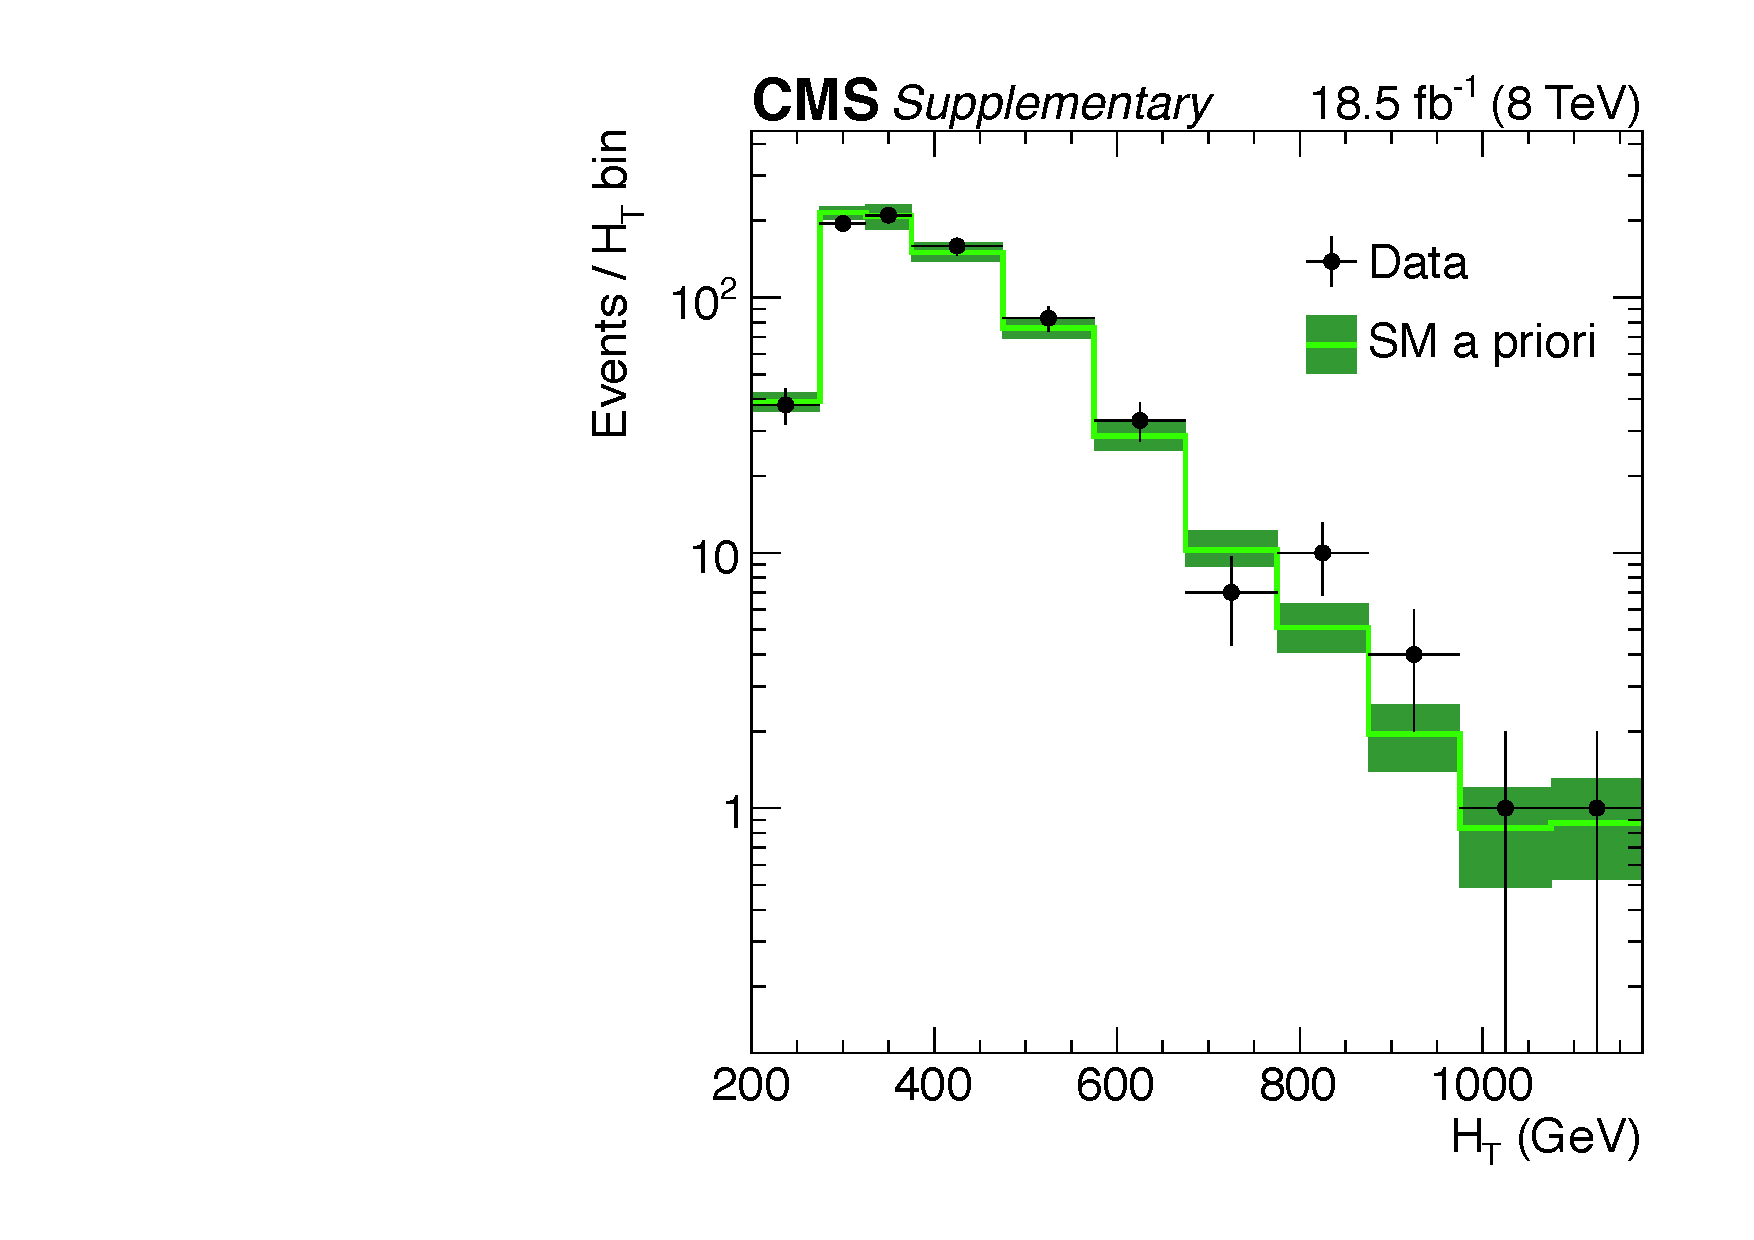
\includegraphics[width=0.7\textwidth]{eq1b_ge4j_prefit_log} 
    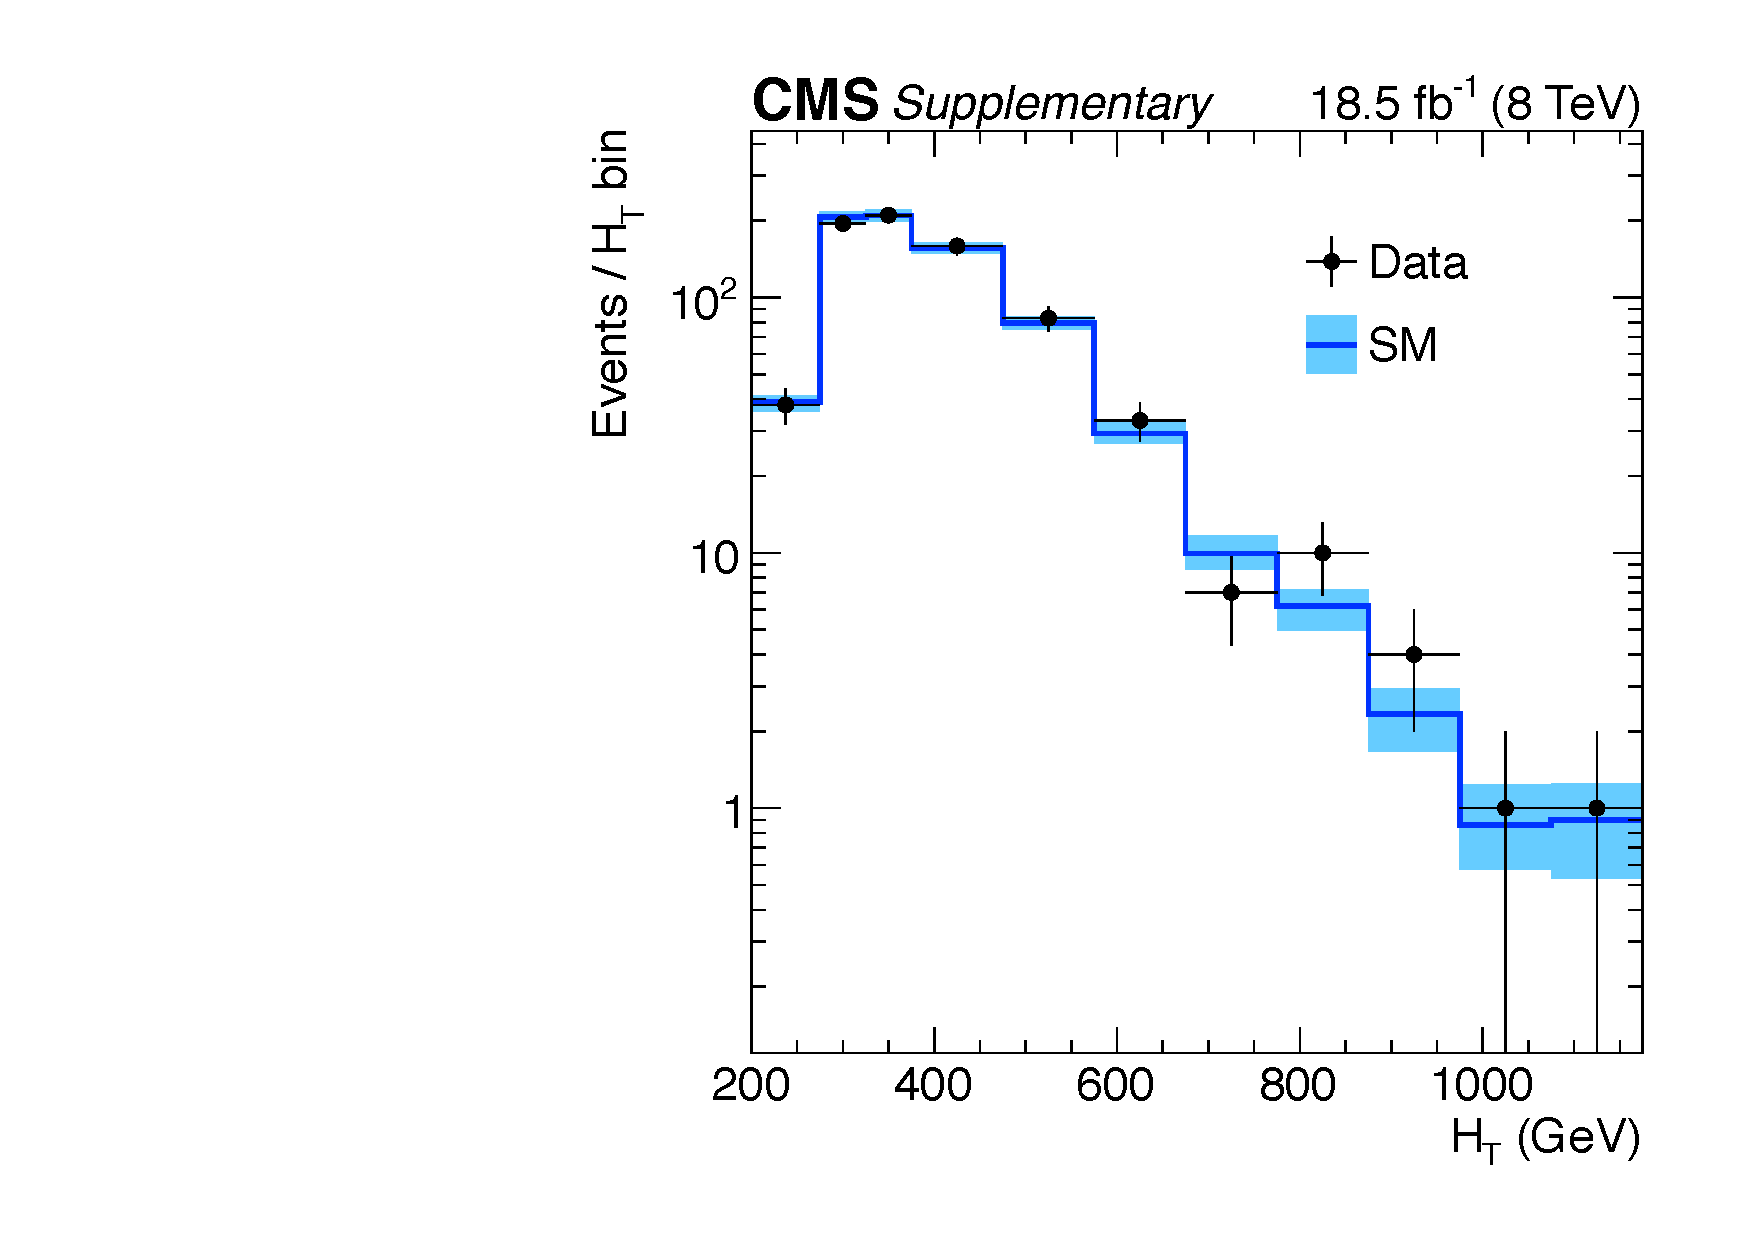
\includegraphics[width=0.7\textwidth]{eq1b_ge4j_postfit_log} \\
    \caption{Candidate signal event yields observed in data (solid
      circles) and SM expectations with their associated uncertainties
      (solid lines with bands) in bins of $H_\text{T}$ for events that
      satisfy $n_\text{jet} \geq 4$ and $n_\text{b} = 1$. (a) SM a
      priori expectations. (b) SM expectations from the fit including
      the signal region. }
  \end{center}
\end{figure}

\clearpage
\begin{figure}[h!]
  \begin{center}
    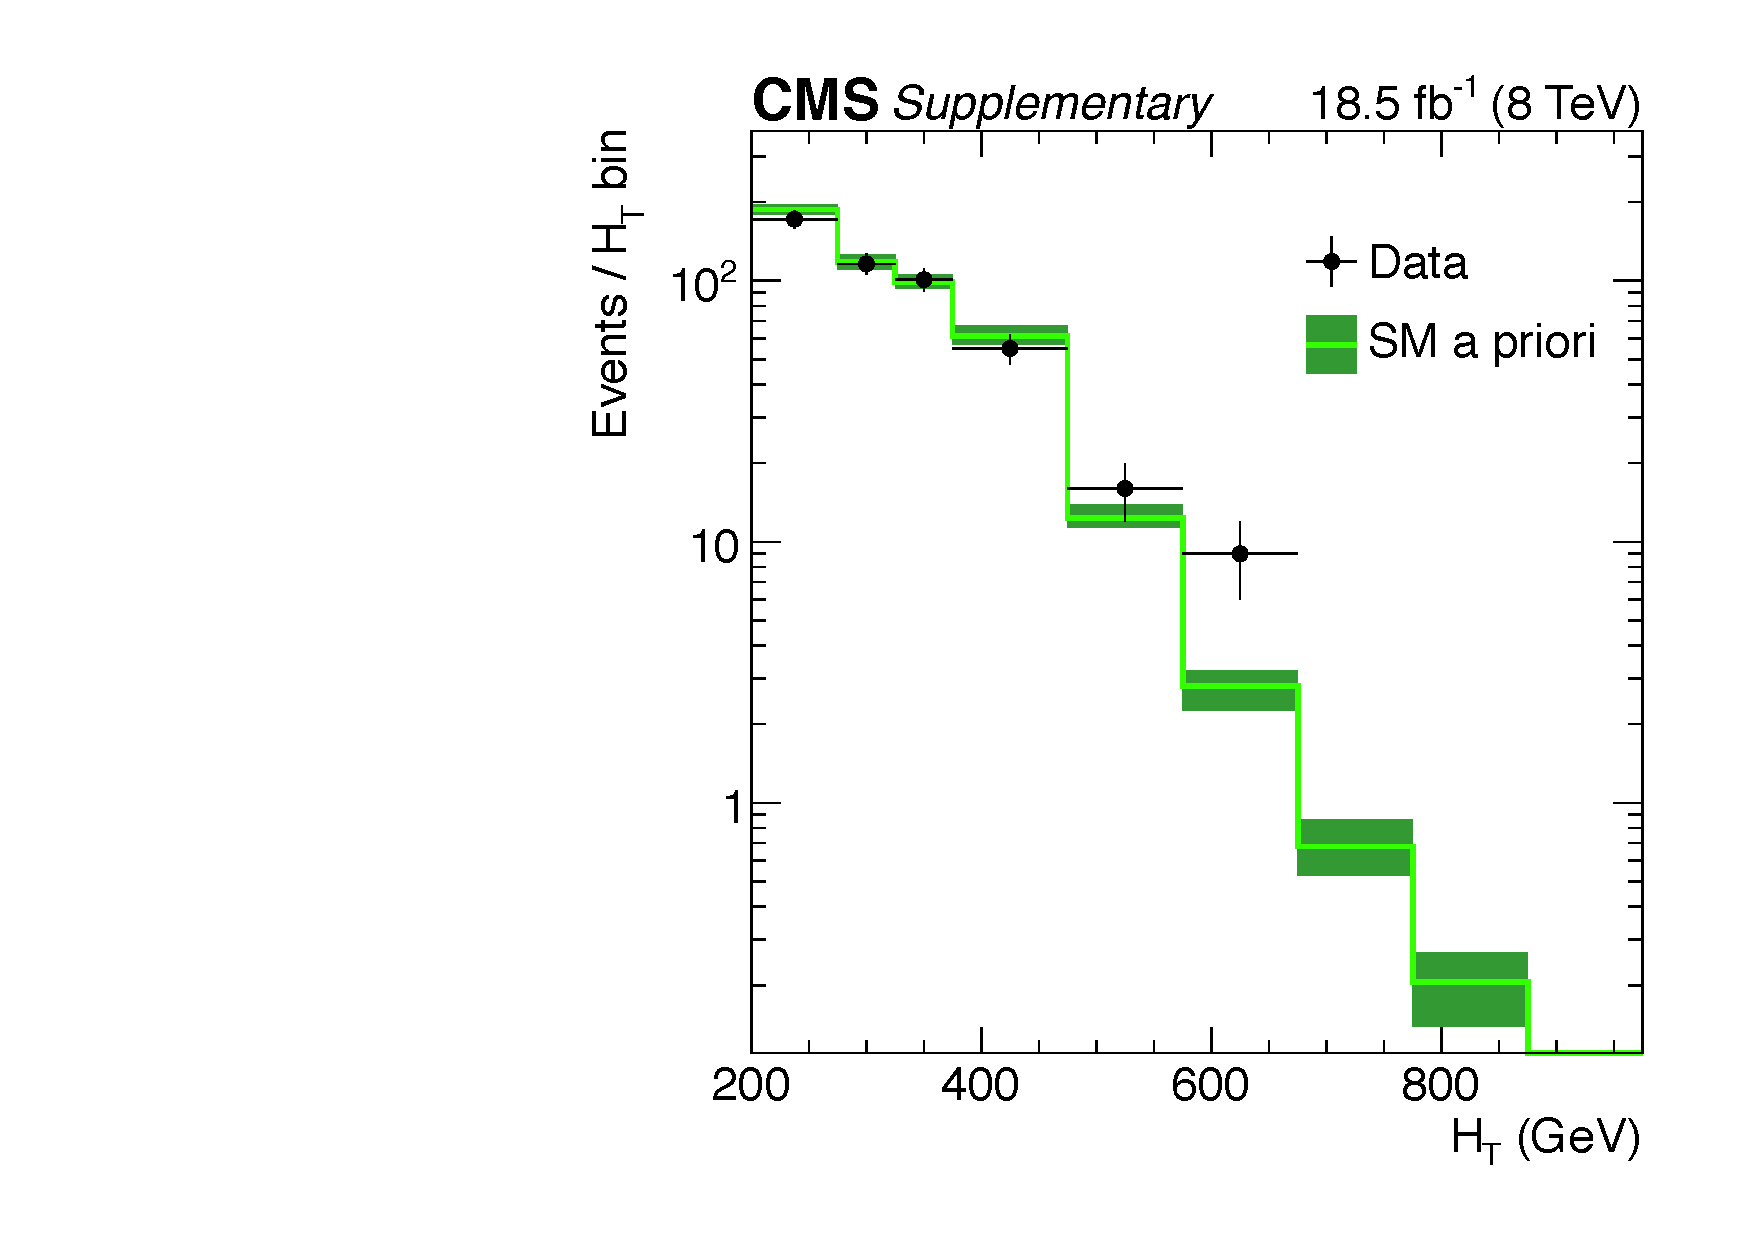
\includegraphics[width=0.7\textwidth]{eq2b_le3j_prefit_log} 
    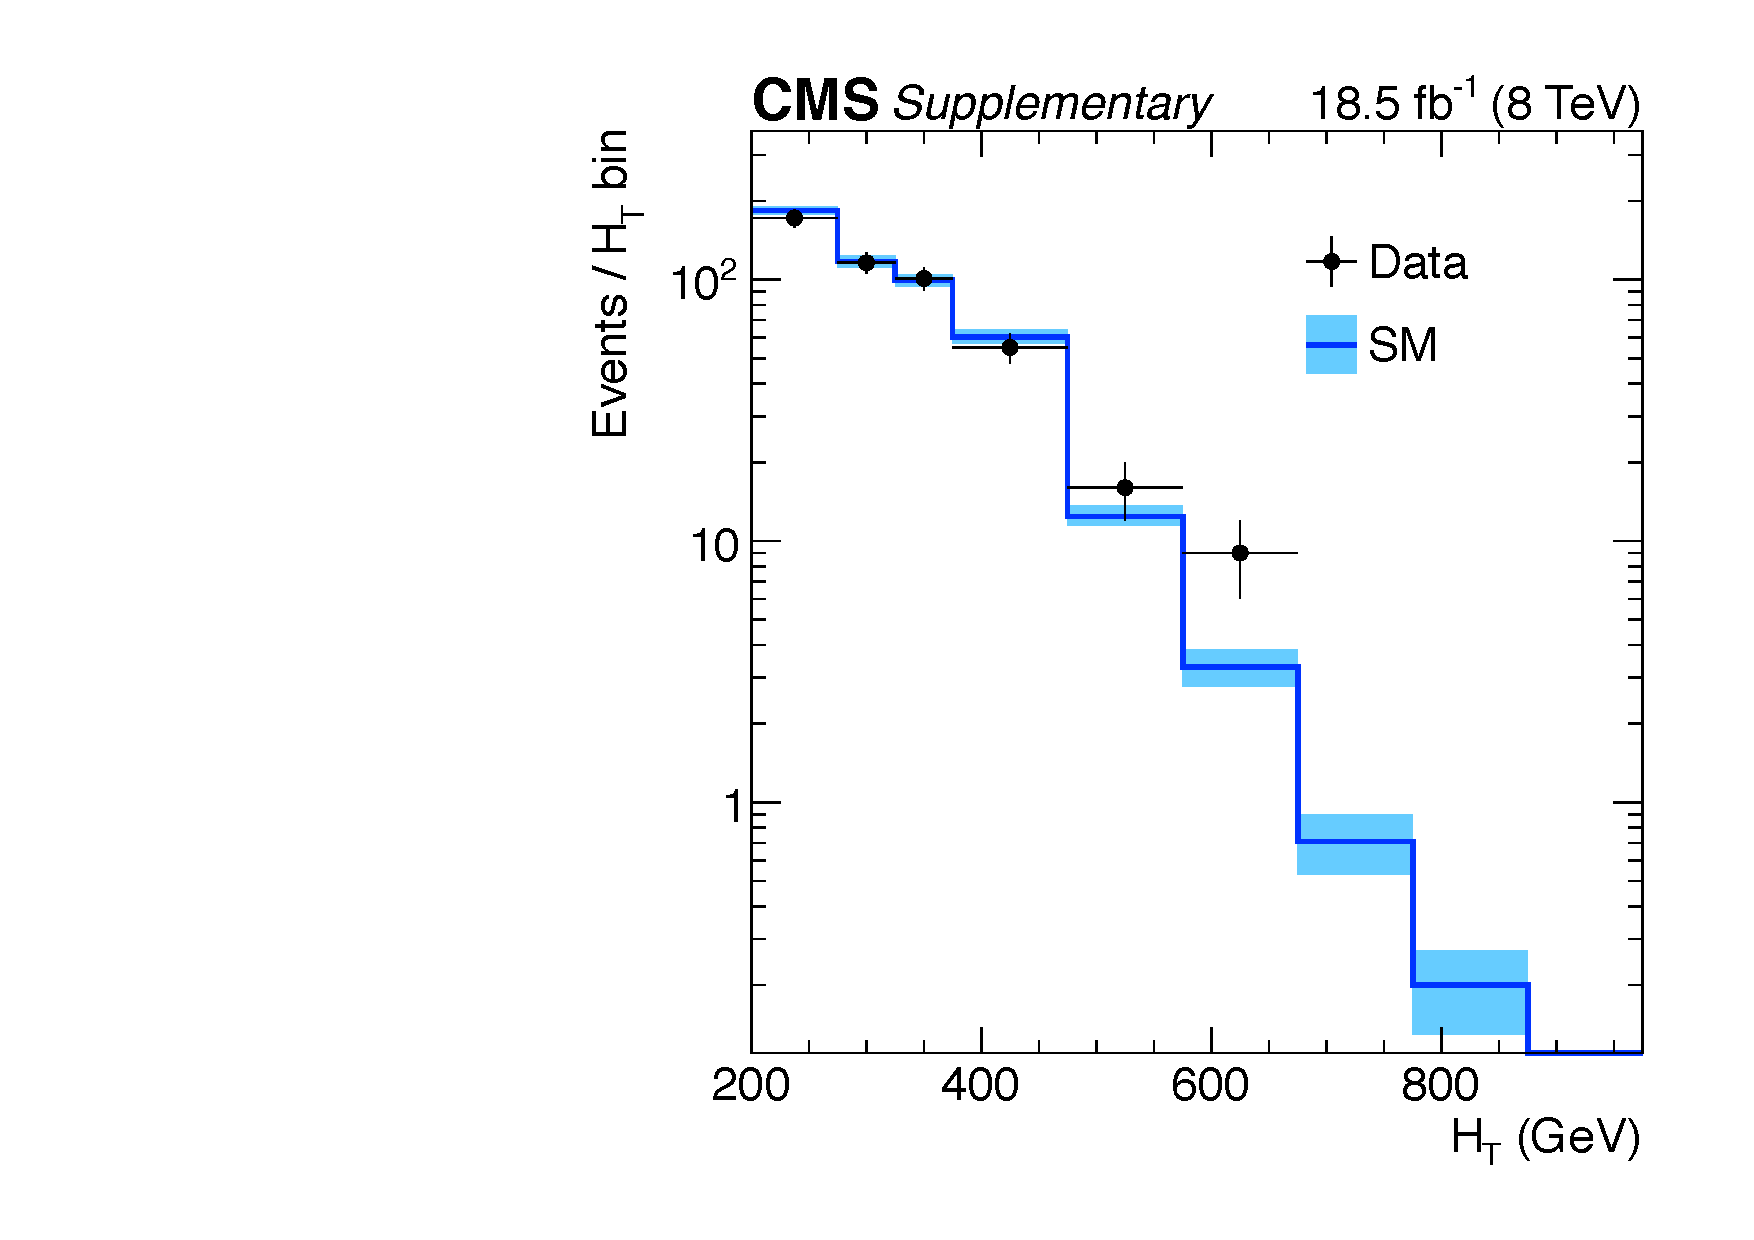
\includegraphics[width=0.7\textwidth]{eq2b_le3j_postfit_log} \\
    \caption{Candidate signal event yields observed in data (solid
      circles) and SM expectations with their associated uncertainties
      (solid lines with bands) in bins of $H_\text{T}$ for events that
      satisfy $2 \geq n_\text{jet} \geq 3$ and $n_\text{b} = 2$. (a)
      SM a priori expectations. (b) SM expectations from the fit
      including the signal region. }
  \end{center}
\end{figure}

\clearpage
\begin{figure}[h!]
  \begin{center}
    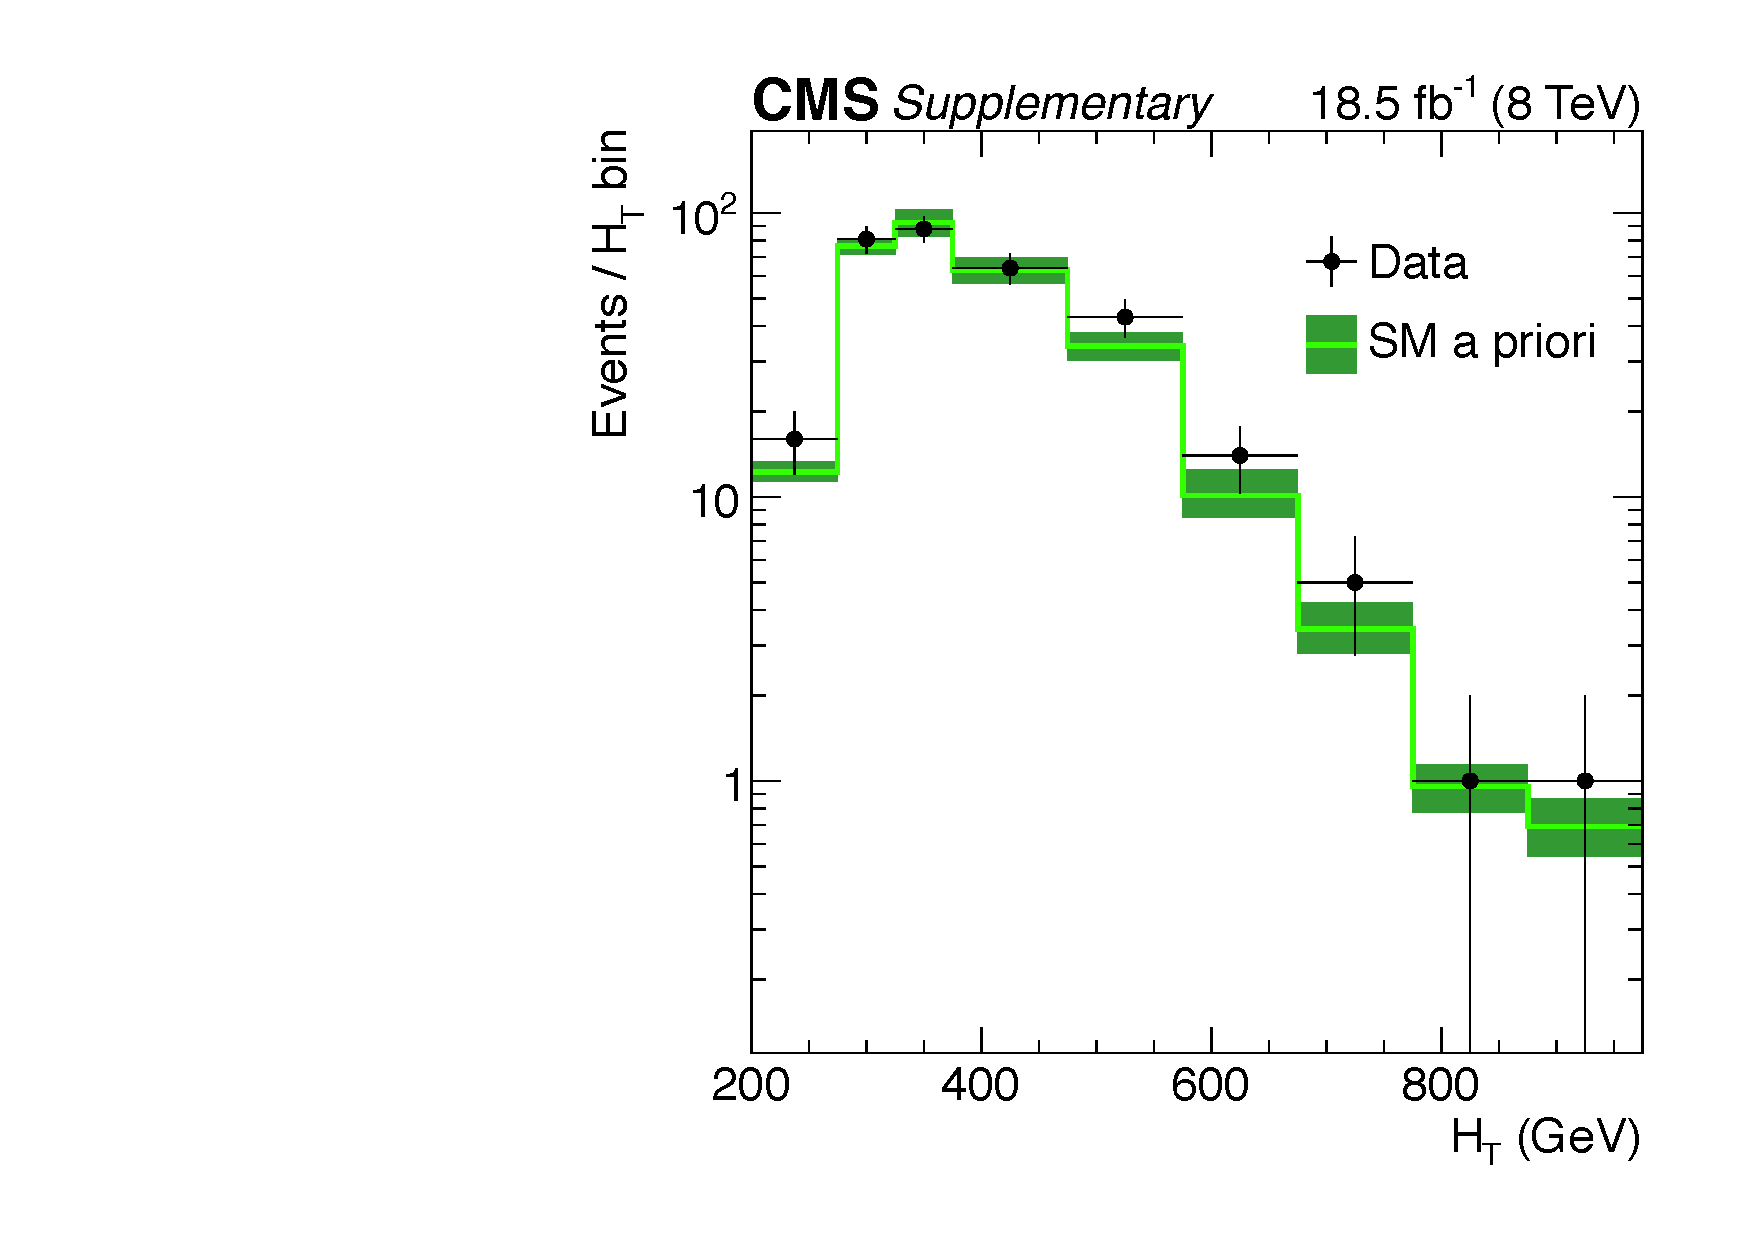
\includegraphics[width=0.7\textwidth]{eq2b_ge4j_prefit_log} 
    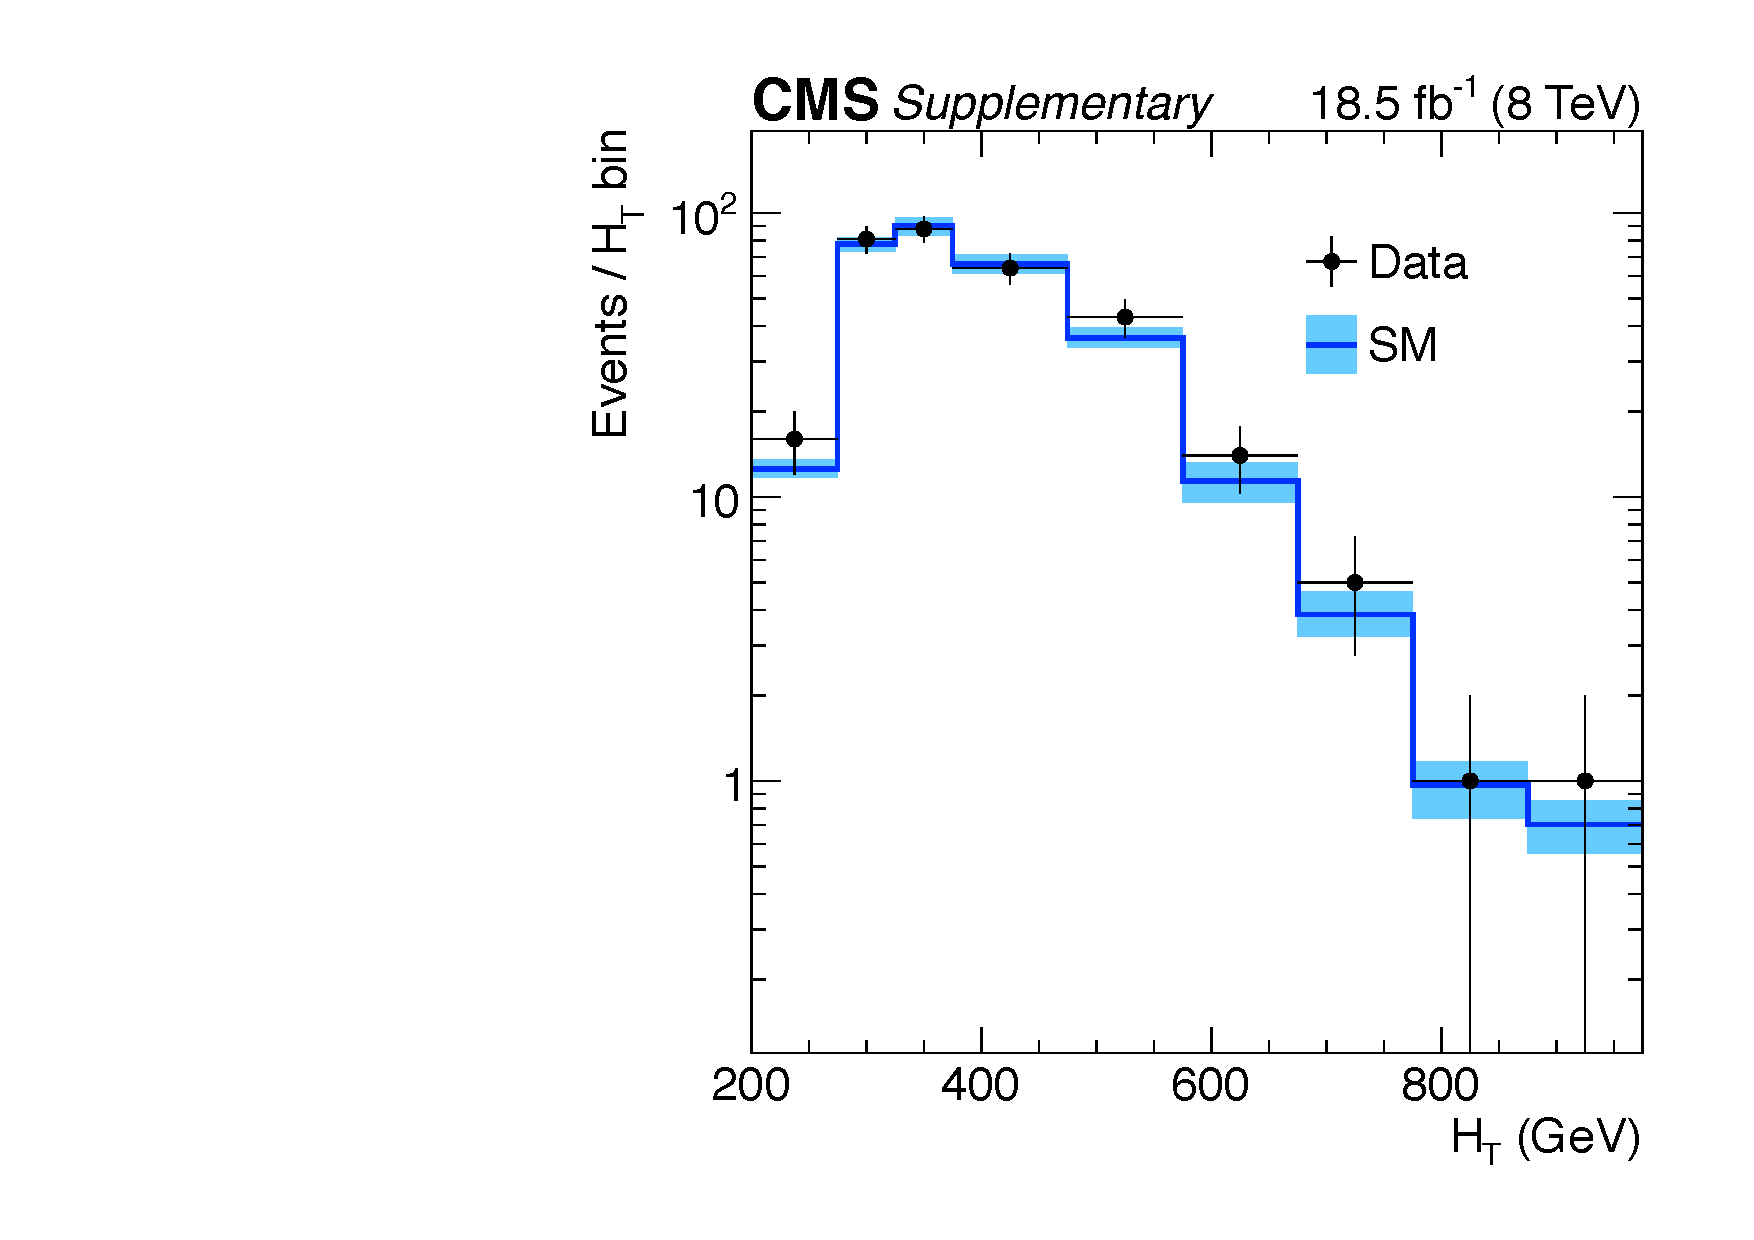
\includegraphics[width=0.7\textwidth]{eq2b_ge4j_postfit_log} \\
    \caption{Candidate signal event yields observed in data (solid
      circles) and SM expectations with their associated uncertainties
      (solid lines with bands) in bins of $H_\text{T}$ for events that
      satisfy $n_\text{jet} \geq 4$ and $n_\text{b} = 2$. (a) SM a
      priori expectations. (b) SM expectations from the fit including
      the signal region. }
  \end{center}
\end{figure}

\clearpage
\begin{figure}[h!]
  \begin{center}
    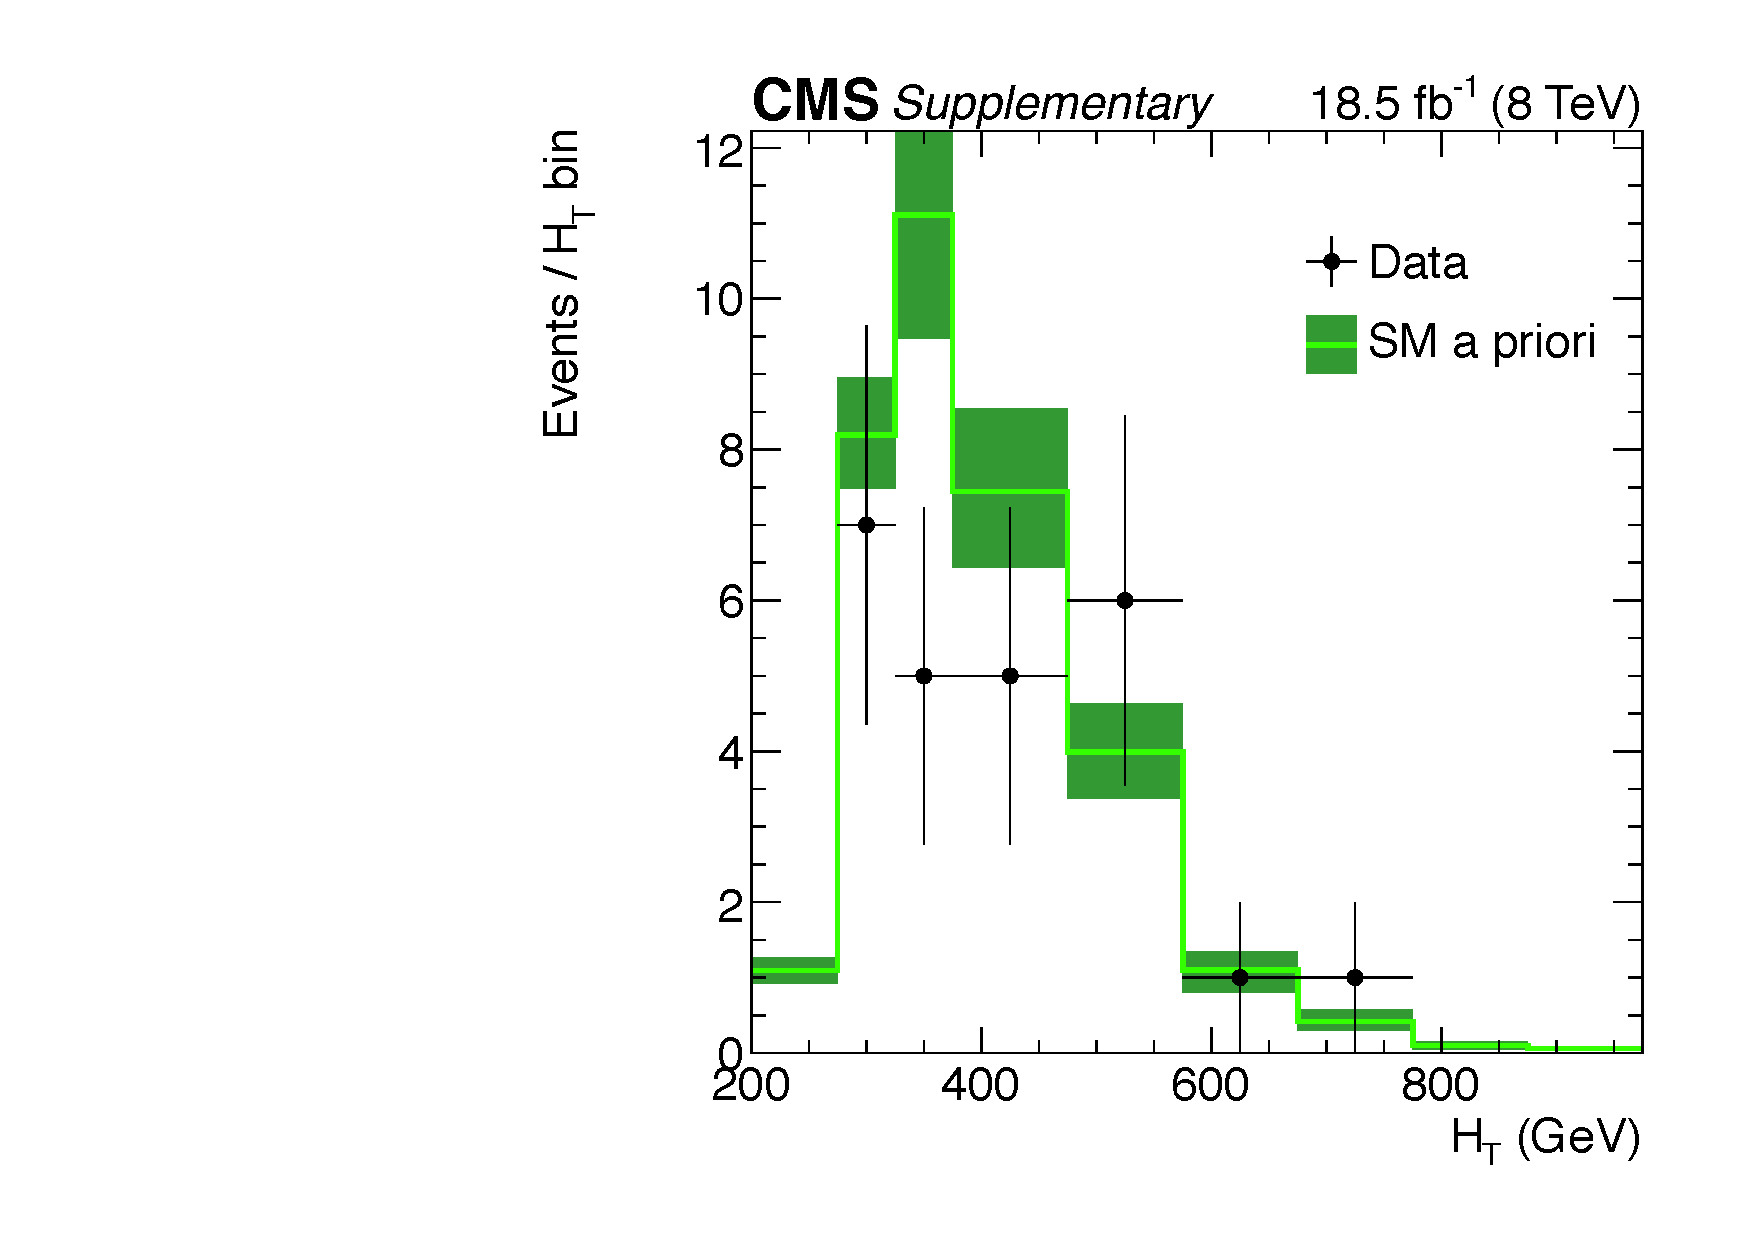
\includegraphics[width=0.7\textwidth]{eq3b_ge4j_prefit_lin} 
    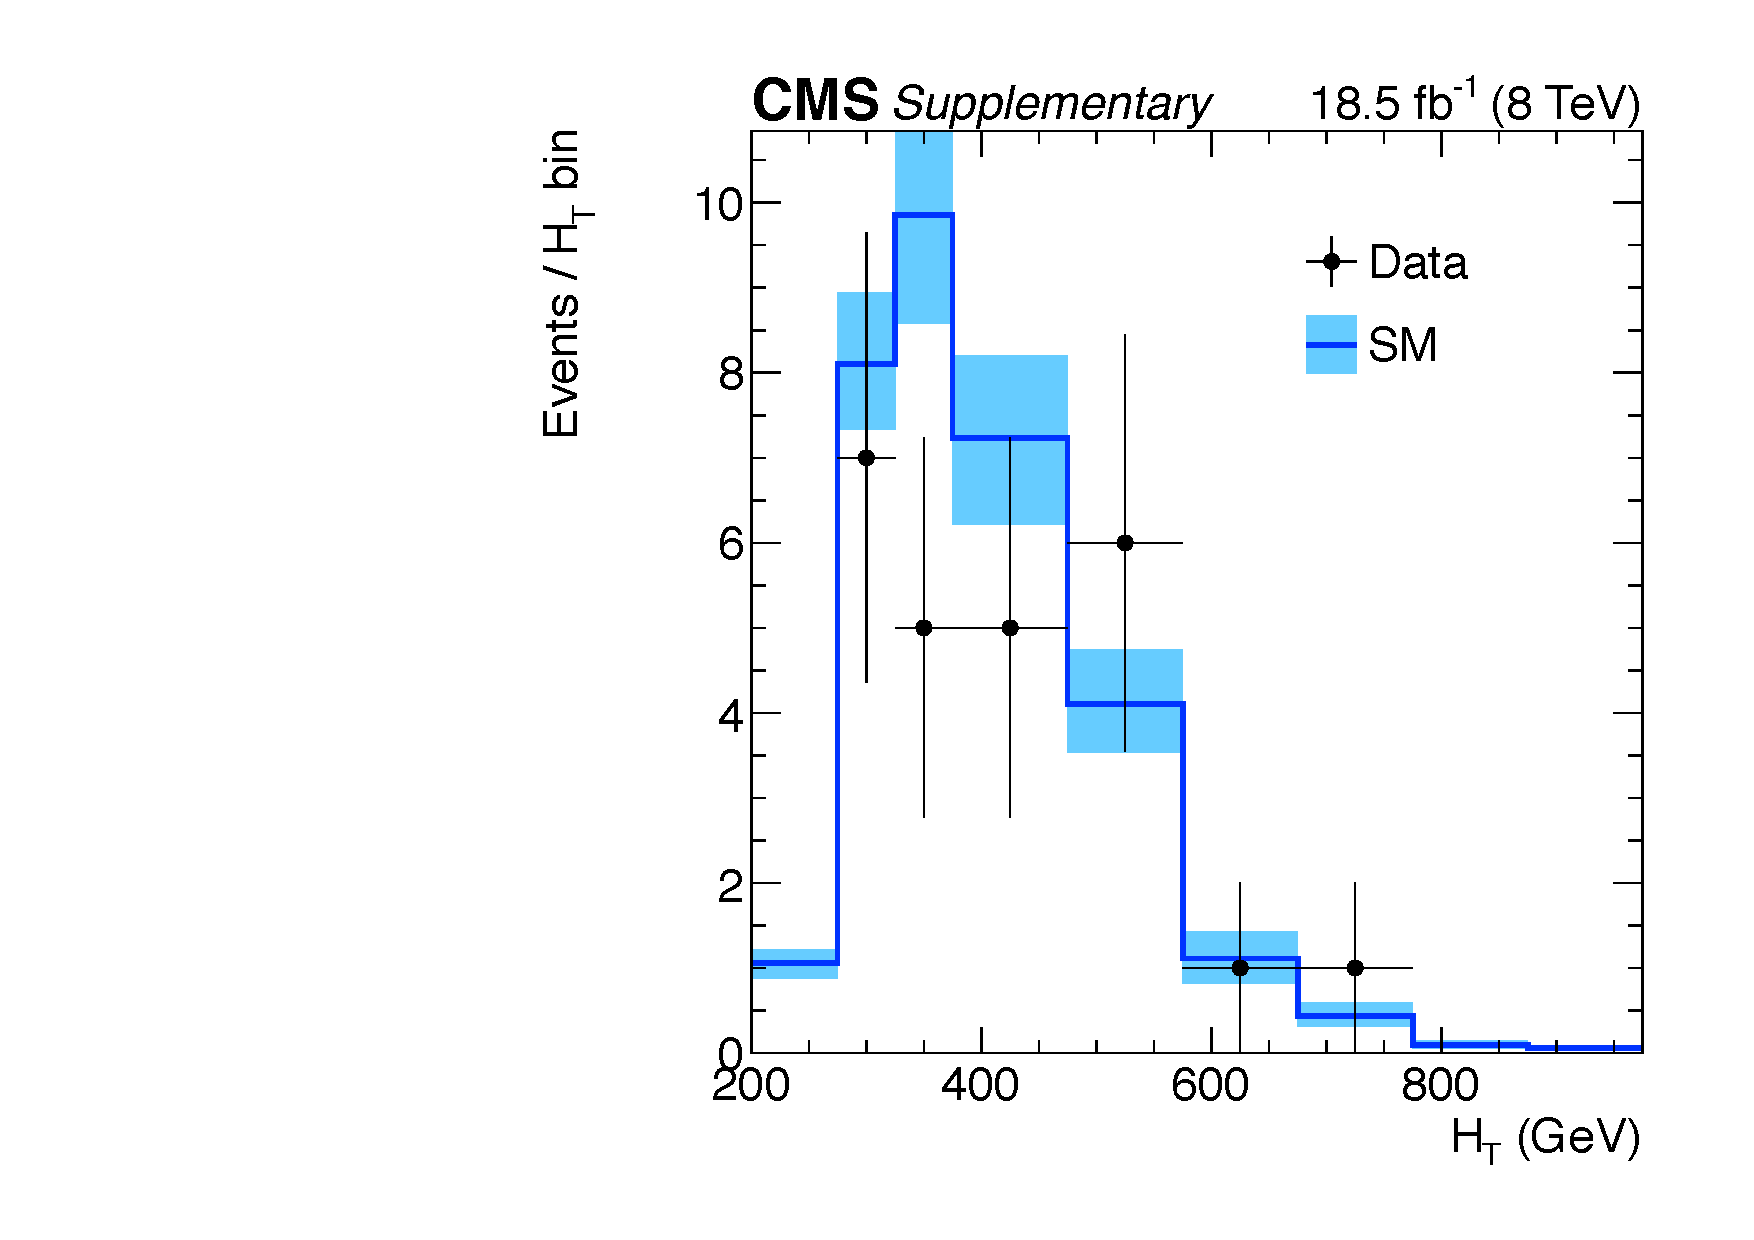
\includegraphics[width=0.7\textwidth]{eq3b_ge4j_postfit_lin} \\
    \caption{Candidate signal event yields observed in data (solid
      circles) and SM expectations with their associated uncertainties
      (solid lines with bands) in bins of $H_\text{T}$ for events that
      satisfy $n_\text{jet} \geq 4$ and $n_\text{b} = 3$. (a) SM a
      priori expectations. (b) SM expectations from the fit including
      the signal region. }
  \end{center}
\end{figure}

\clearpage
\begin{figure}[h!]
  \begin{center}
    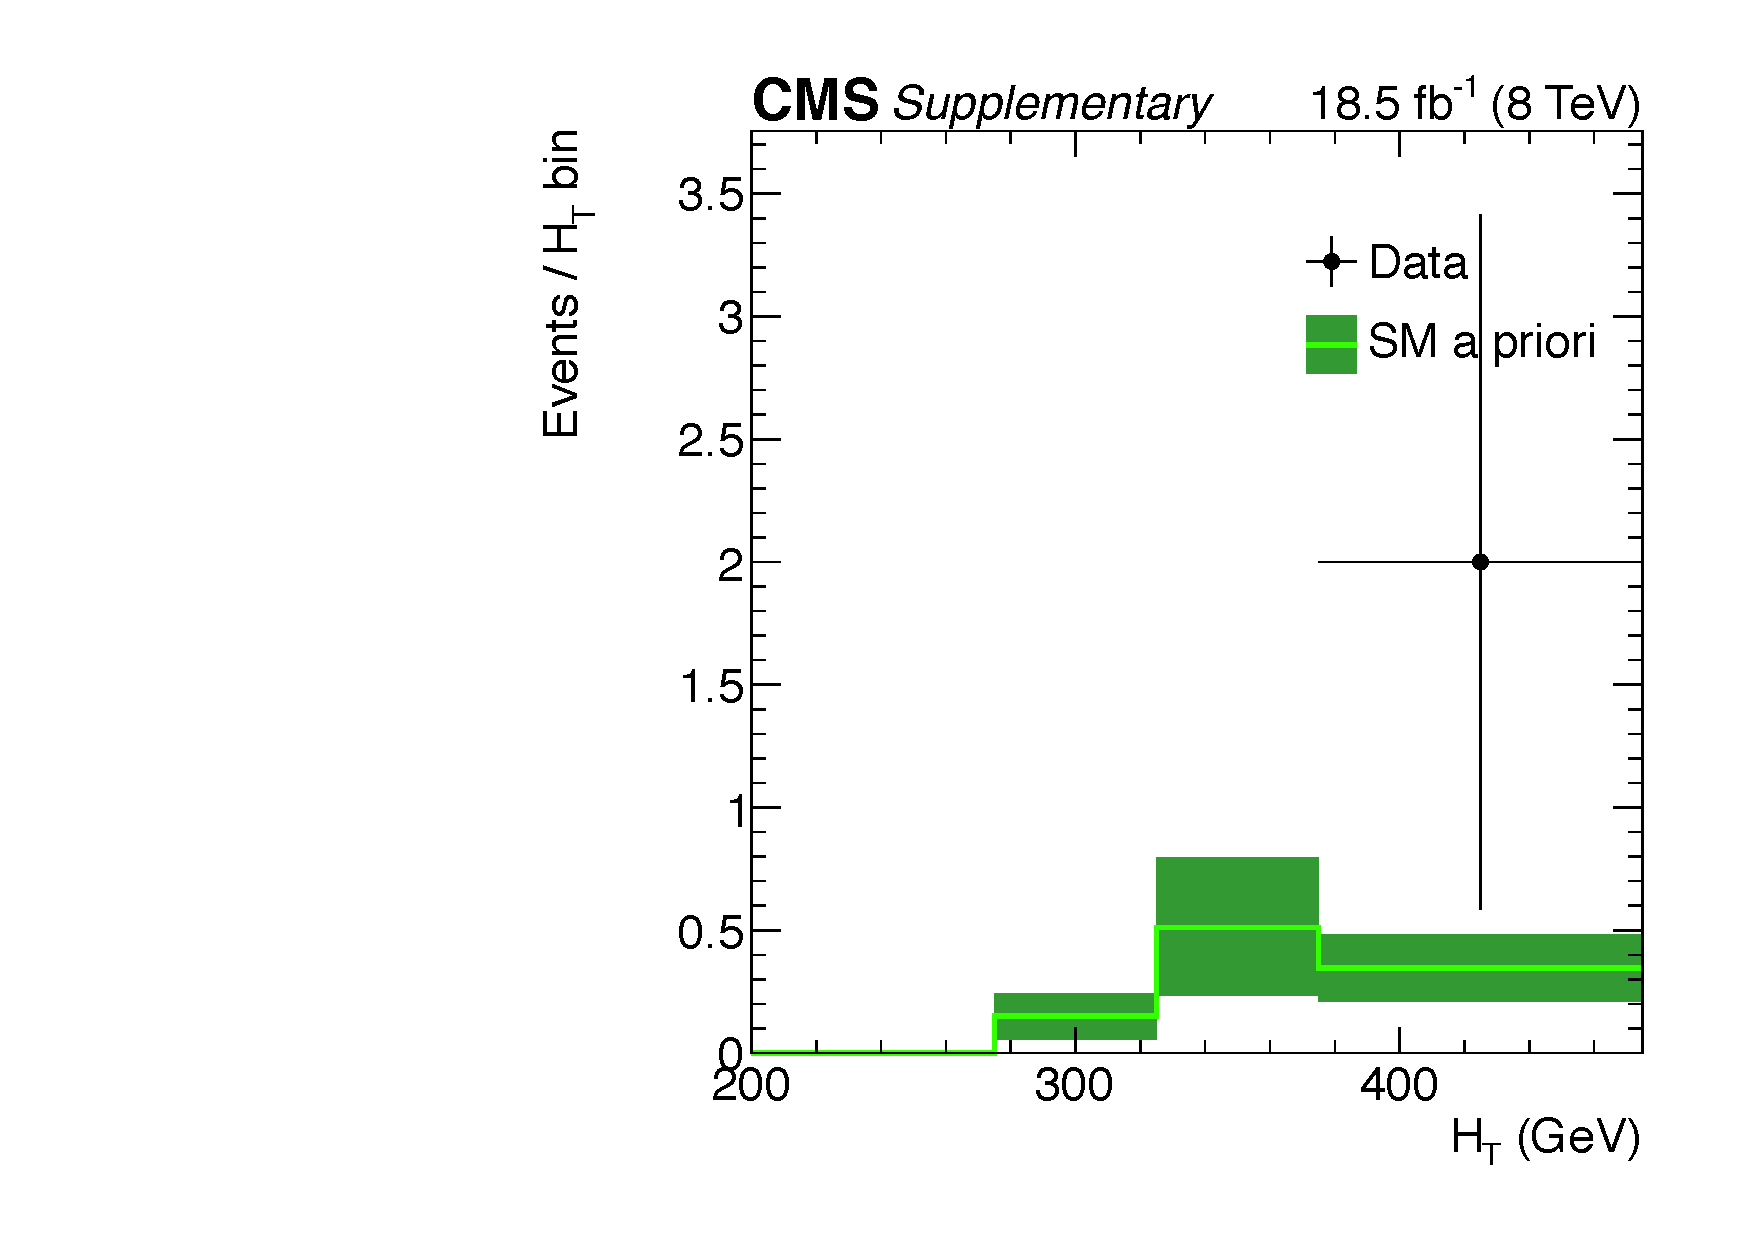
\includegraphics[width=0.7\textwidth]{ge4b_ge4j_prefit_lin} 
    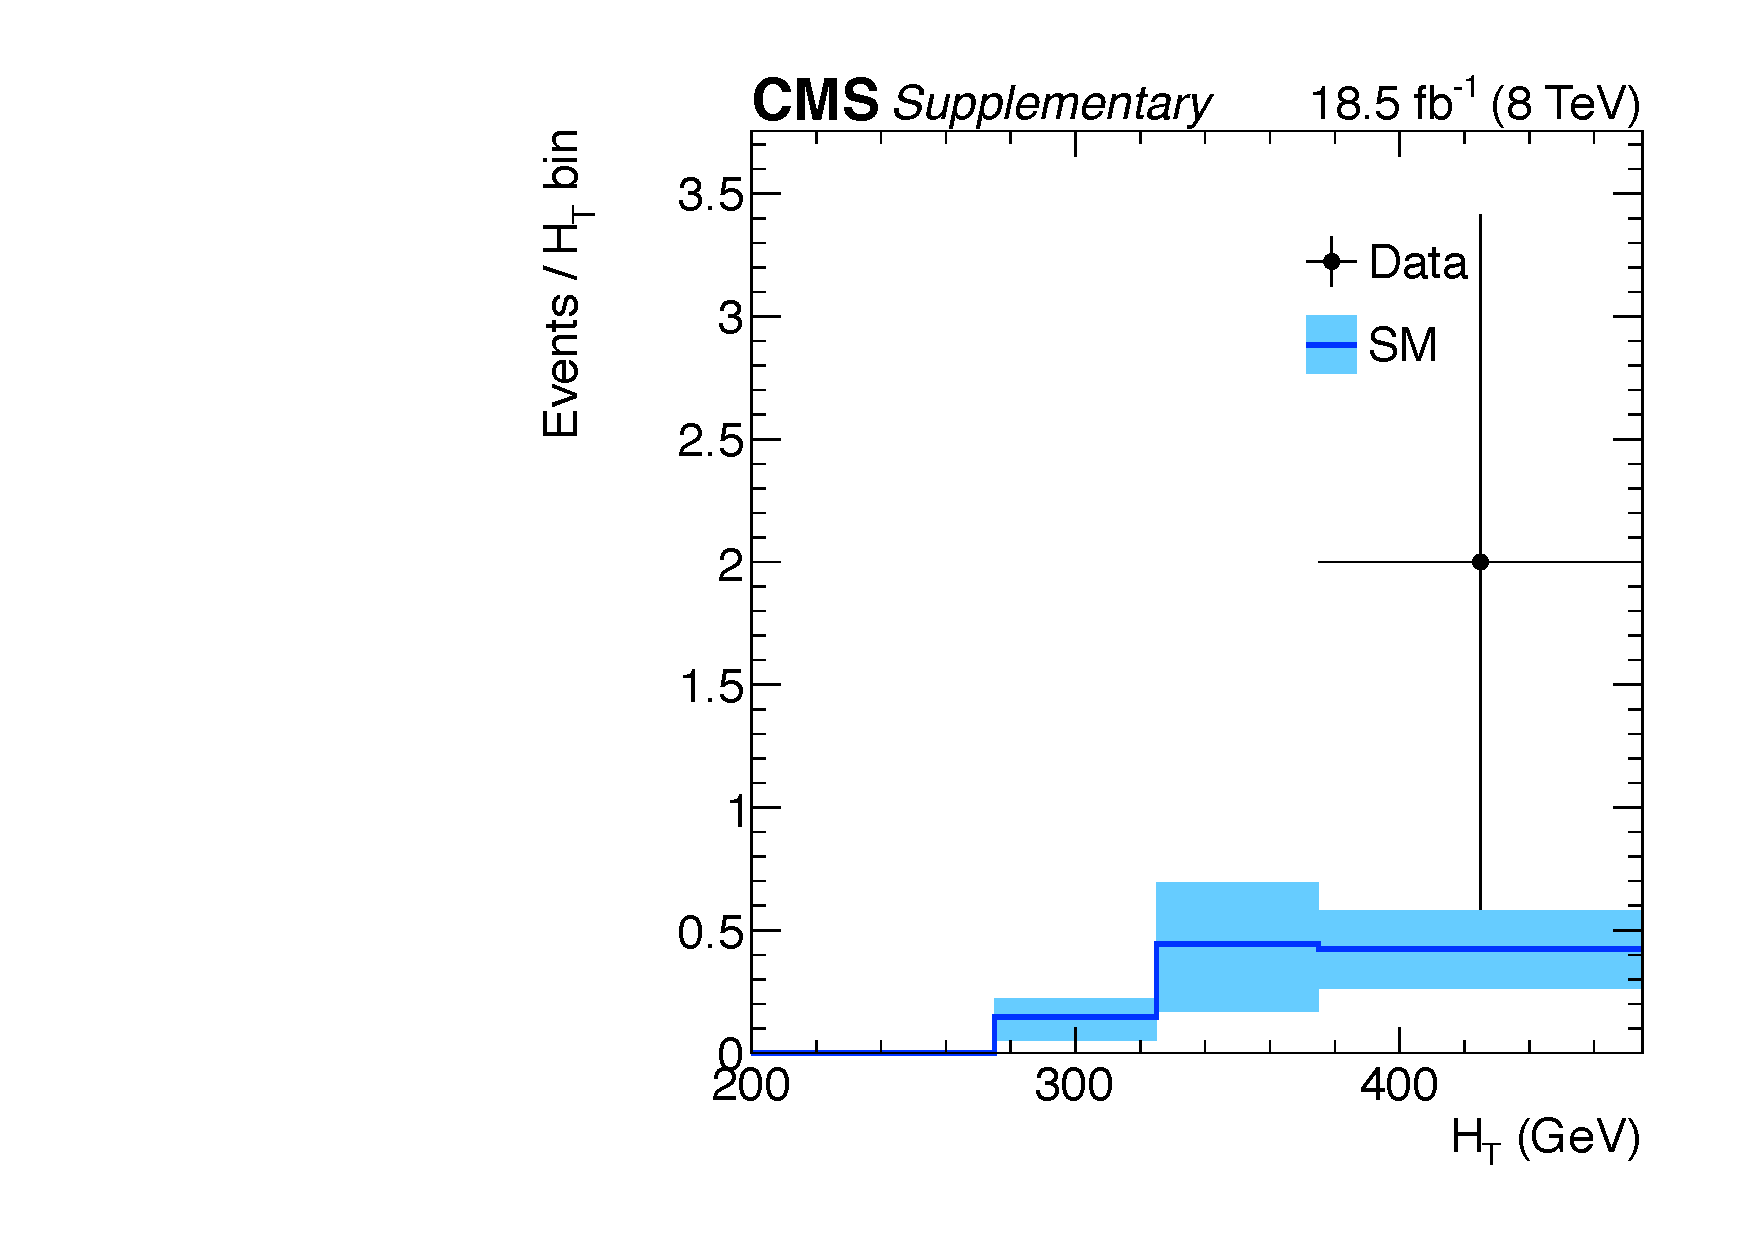
\includegraphics[width=0.7\textwidth]{ge4b_ge4j_postfit_lin} \\
    \caption{Candidate signal event yields observed in data (solid
      circles) and SM expectations with their associated uncertainties
      (solid lines with bands) in bins of $H_\text{T}$ for events that
      satisfy $n_\text{jet} \geq 4$ and $n_\text{b} \geq 4$. (a) SM a
      priori expectations. (b) SM expectations from the fit including
      the signal region. }
  \end{center}
\end{figure}

\clearpage
\newcommand{\n}{\phantom{1}}
\newcommand{\nn}{\phantom{10}}
\begin{table}[h!]
  \caption{Cumulative signal acceptance times efficiency (\%) for the
    event selection criteria that define the signal region, for models
    involving the pair production of top squarks and the following
    decay modes: a loop-induced, flavour-changing neutral current
    decay to a charm quark and a neutralino, $\PSQt \to
    \PQc\PSGczDo$, or a four-body decay, $\PSQt \to \PQb f{\bar{f}'}
    \PSGczDo$, where b is a bottom quark with $f$ and $\bar{f}'$ 
    fermions from, for example, an off-shell W boson decay. The models
    are defined by the masses (GeV) of the top squark and the
    neutralino, ($m_{\,\PSQt}$, $m_{\PSGczDo}$). 
  } 
  \centering
  \renewcommand*{\arraystretch}{1.2}
  \begin{tabular}{ lllll }
    \hline
    Event selection                                                           & \multicolumn{4}{c}{Model}               \\ 
    \cline{2-5}
                                                                              & $\PSQt\to\PQc\PSGczDo$ 
                                                                              & $\PSQt\to\PQc\PSGczDo$  
                                                                              & $\PSQt \to {\PQb f{\bar{f}'}} \PSGczDo$ 
                                                                              & $\PSQt \to {\PQb f{\bar{f}'}} \PSGczDo$ \\
                                                                              & (250,240) 
                                                                              & (250,170) 
                                                                              & (250,240)                               
                                                                              & (250,170)                               \\
                                                                  \hline
    --                                                                        & 100     & 100     & 100     & 100       \\
    $n_\text{jet} \geq 2$ ($E_\text{T} > 50\GeV$, $|\eta| < 3.0$)             & \n13    & \n60    & \n11    & \n32      \\
    Event cleaning                                                            & \n13    & \n60    & \n11    & \n32      \\
    $E_\text{T}^\text{miss}$ cleaning                                         & \n11    & \n44    & \nn9.1  & \n21      \\
    Lepton and photon vetoes                                                  & \n11    & \n44    & \nn9.1  & \n17      \\
    Highest $E_\text{T}$ jet: $E_\text{T} > 100\GeV$                          & \nn7.4  & \n25    & \nn6.0  & \nn8.7    \\
    Highest $E_\text{T}$ jet: $|\eta| < 2.5$                                  & \nn7.0  & \n24    & \nn5.7  & \nn8.4    \\
    Next-to-highest $E_\text{T}$ jet: $E_\text{T} > 100\GeV$                  & \nn2.3  & \nn8.9  & \nn1.6  & \nn2.2    \\
    $n_\text{jet}^\text{forward} = 0$ ($E_\text{T} > 50\GeV$, $|\eta| > 3.0$) & \nn2.3  & \nn8.7  & \nn1.6  & \nn2.2    \\
    Single isolated track veto                                                & \nn2.1  & \nn8.0  & \nn1.5  & \nn1.7    \\
    $\Delta\Phi^{*}_\text{min} > 0.3$                                         & \nn1.8  & \nn5.4  & \nn1.4  & \nn0.93   \\
    $H_\text{T}^\text{miss}/E_\text{T}^\text{miss} < 1.25$                    & \nn1.7  & \nn4.5  & \nn1.2  & \nn0.68   \\
    $H_\text{T} > 375\GeV$                                                    & \nn0.90 & \nn2.1  & \nn0.55 & \nn0.37   \\
    $\alpha_\text{T} > 0.55$                                                  & \nn0.45 & \nn0.40 & \nn0.26 & \nn0.08   \\
    \hline
  \end{tabular}
\end{table}

%\bibliography{auto_generated}
